\chapter{Discovering the Optimum Model and Increasing Dataset Size}
\label{sec:bestmodel}
% Discuss updates since Prelim, including increasing dataset size and discovery of best model

Various issues arise in the preceding chapters regarding the classification system developed and dataset compiled.
A brief list of such issues includes:

\begin{itemize}
	\item Limited labeled dataset
	\item Restricted generalization ability of the model
	\item Lack of integration of recent developments in image-based machine learning techniques
\end{itemize}

As previously discussed, the initial dataset includes, in total, roughly 1,200 weather radar images.
This dataset was compiled by the author's careful inspection of hundreds of thousands of images and labeled by hand when a particular meteorological phenomena or precipitation regime was present.
The data corpus was constructed of scans from one X-band radar, located in Midlothian, TX, with time coverage between January 2016 to December 2017.
Given that plan-position indicator (PPI) scans are produced at the 1 degree elevation every minute, there are roughly 500,000 scans available each year.
Even with diligent searching and labeling, many potentially valuable radar scans representing phenomena of interest will be missed.

Part of the inspiration for this work, and indeed a major goal, however, was to be able to apply a "less-educated" model to new data, produce what may be referred to as "less-educated guesses" as to class membership on said new data, and allow a human expert the ability to peruse these guesses and correct mistakes made in terms of false positives and false negatives.
This process greatly reduces the time taken to label the many thousands of candidate images and generates an opportunity to increase the dataset size by an order of magnitude.

The second item in the list above goes hand-in-hand with the first item, in that in order to improve the generalization ability of the model, we must be able to train the model using many more representations of classes of interest.
To do this, we must include more data.

\begin{figure}[h]
	\centering
	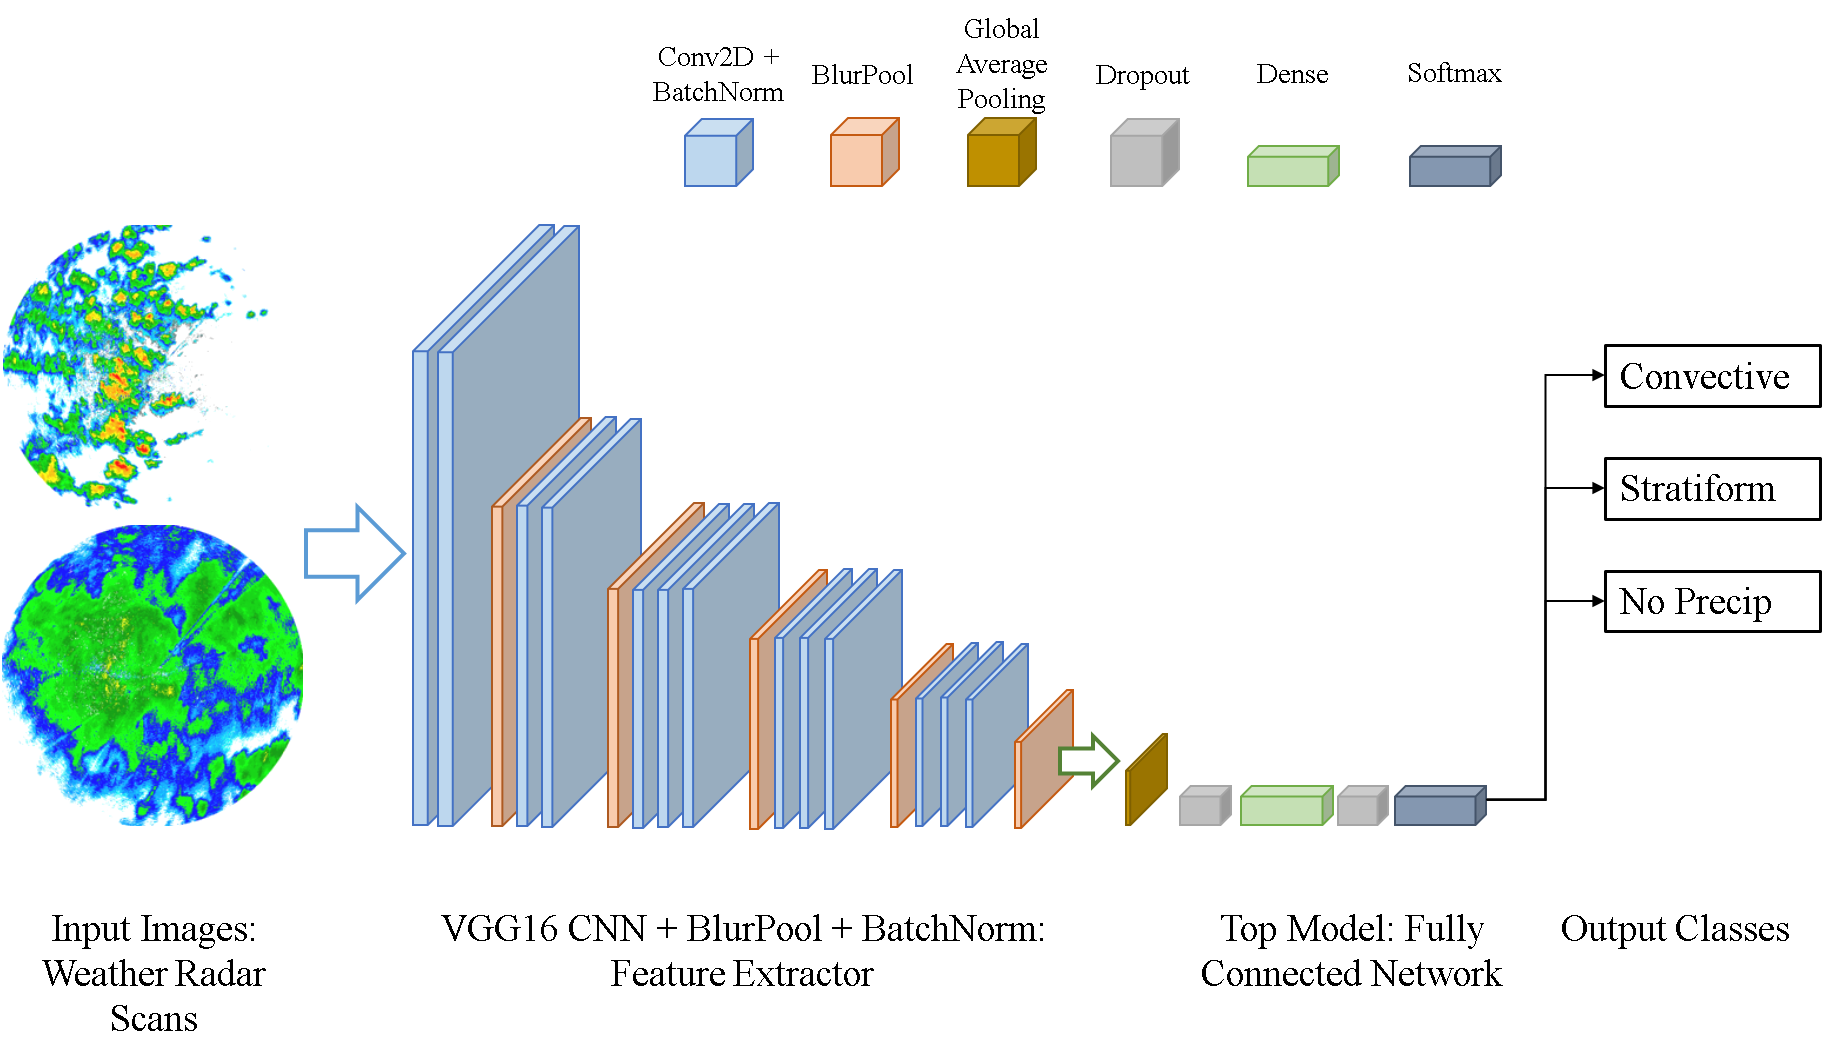
\includegraphics[width=\textwidth]{./thesis_code/plots/DL-workflow.png}
	\caption{Complete end-to-end deep learning architecture devised in this chapter. Note that convolution layers now include batch normalization, while downsampling layers are formed by the new BlurPool layer. These two are tuneable parameters in this architecture, and we tested many configurations to find the best set of parameters and hyperparameters.}
	\label{fig:end-to-end}
\end{figure}

The third item can be used to assist the second item as well. Computer vision, transfer learning, and machine learning in general are currently some of the most active areas of research in science as a whole.
The tools that are being developed, and indeed, that have been developed, can find application in almost every field, and each field in turn can offer insight into improving the tools themselves.
It is essentially impossible for any one researcher or team of researchers to stay abreast of every relevant development related to their field.
However, leveraging insights made from recent discoveries remains useful, important, and essential for any effort in this field.

To that end, we propose a set of experiments to determine the optimal model to use for our transfer learning procedure by incorporating recent discoveries from the field into our deep learning model architecture, and testing each variation on a consistent dataset to determine the best architecture.
The following sections in this chapter detail the efforts made to increase the dataset size, descriptions of the additional model layers, and present the results of the set of experiments that yields the optimum model, given these alterations and improvements.
We illustrate that the optimum model from the tested configurations is shown in the end-to-end architecture diagram in Figure \ref{fig:end-to-end}.

\section{Increased Dataset Size}
\label{sec:bestmodel_dataset}

\section{BlurPool}
\label{sec:bestmodel_blurpool}

A dataset must include many representations of the desired phenomena of interest in order to allow better generalization on test sets.
In the specific case of weather radar data, however, it is likely to see scans that are highly visually similar to one another when successive scans are recorded in one minute intervals, as the images in this study are produced.
This high level of inter-image intercorrelation may lead to instances of overfitting, if the training dataset is not large enough to present many uncorrelated events, as well as many scans for each event.
Storms and weather precipitation events will tend to move slowly across the high-resolution, large geographic sampling area present in each scan, leading to the same or similar echoes occurring in tens of successive scans as represented in Figure \ref{fig:bestmodel_translation}.
It is thus desirable to not only encourage generalizability to unseen data in a particular classifier, but in this case, to also be resilient to image object translation.

\begin{figure}[h]
	\centering
	\begin{subfigure}[b]{0.3\textwidth}
		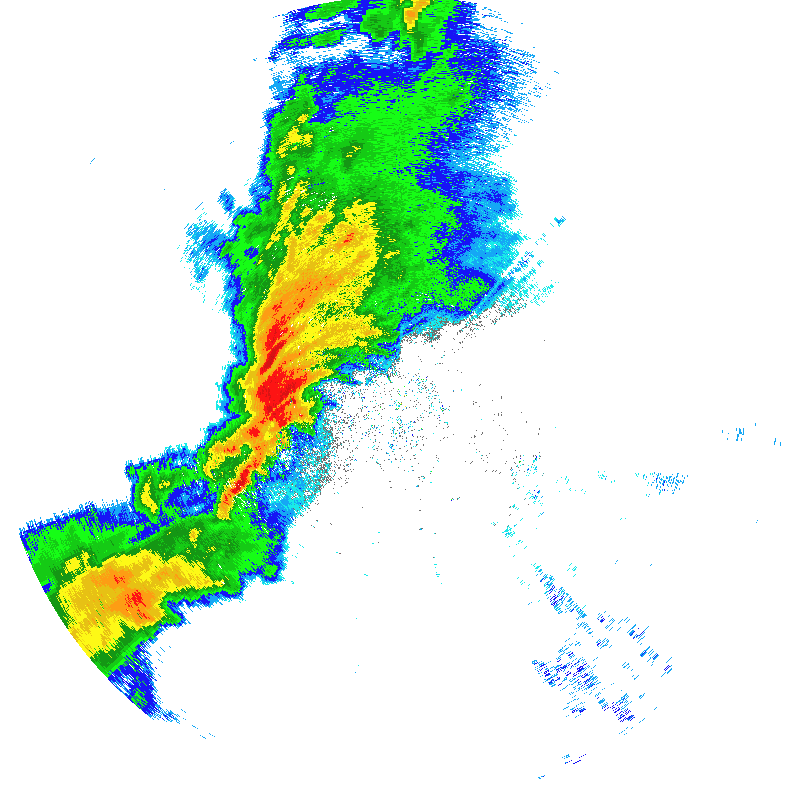
\includegraphics[width=\textwidth]{./thesis_code/plots/midlothian.tx-20180421-235038-ref.png}
		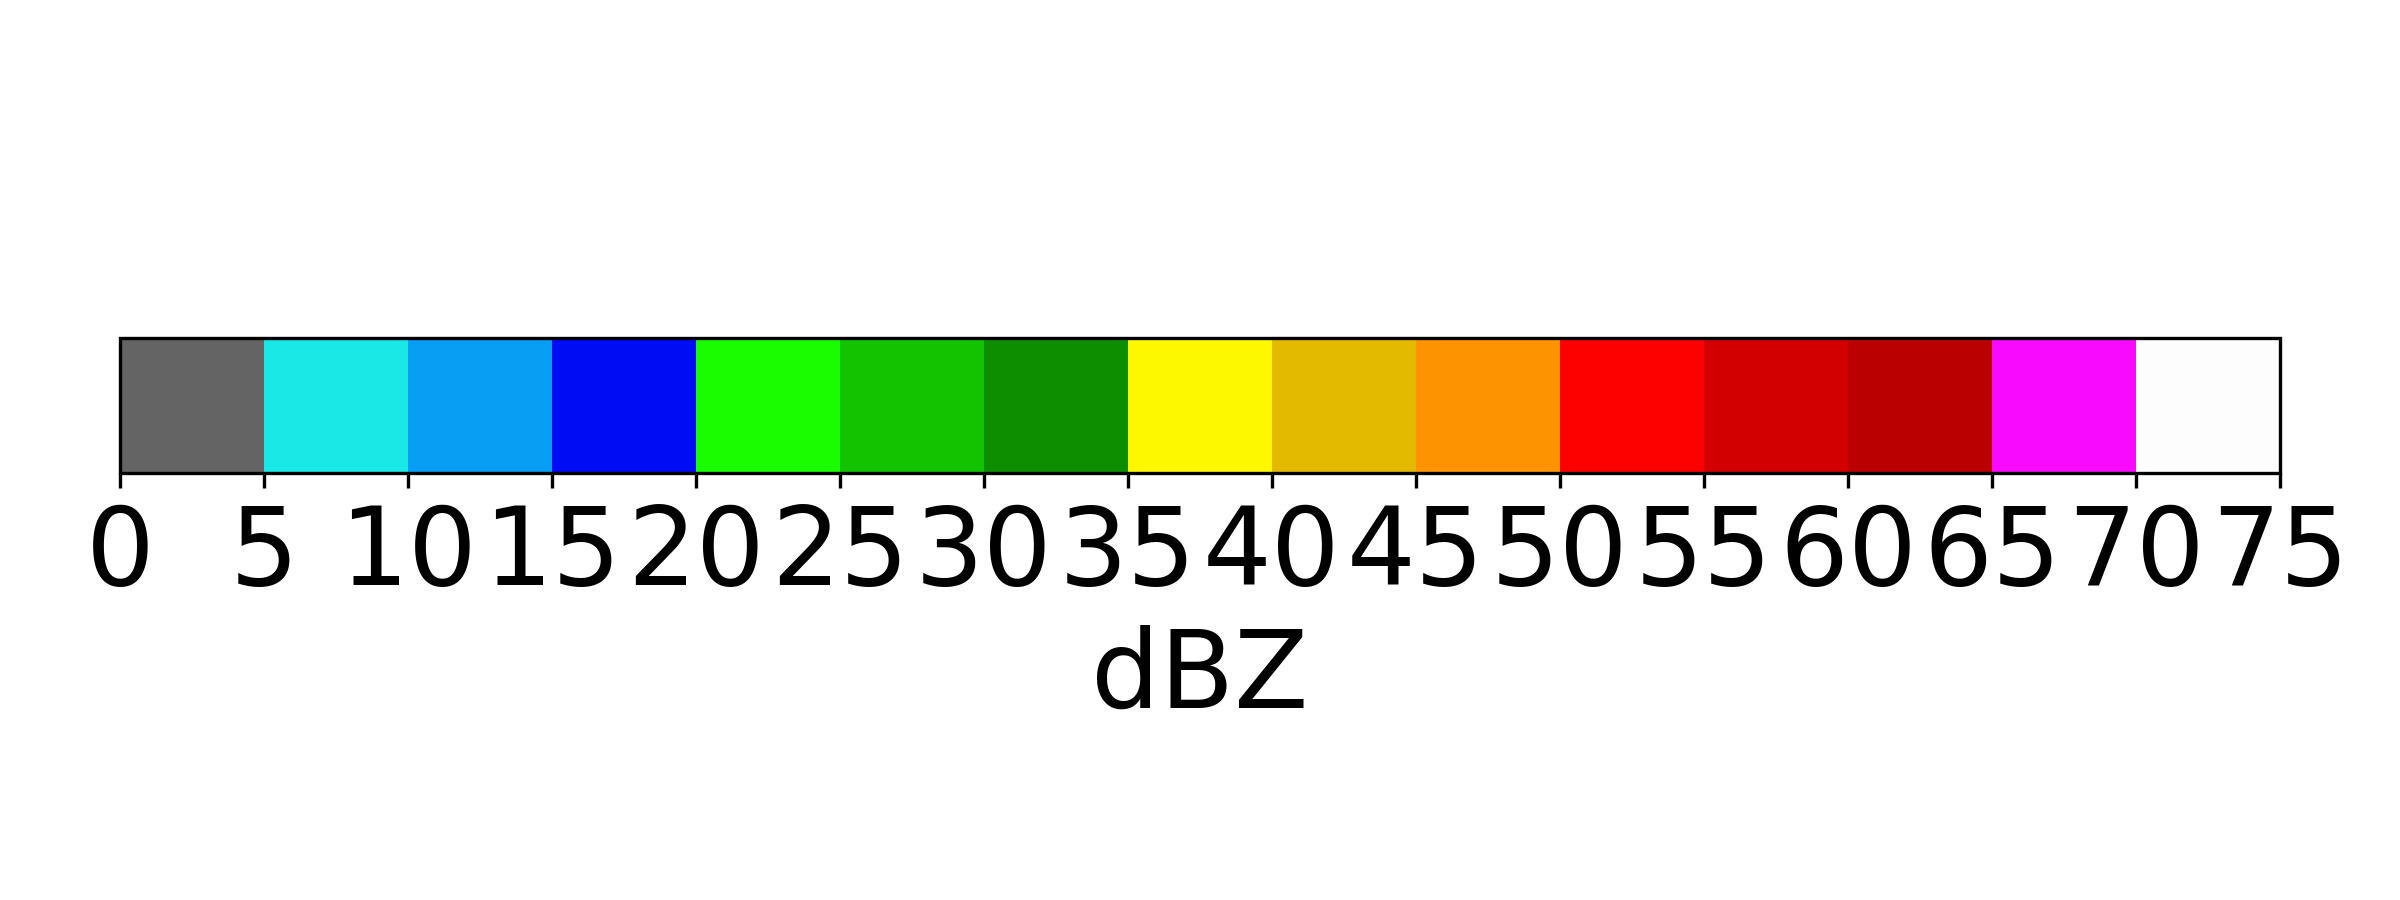
\includegraphics[width=\textwidth]{./thesis_code/plots/dfw_colormap.png}
		\caption{2018-04-21 23:50:38 UTC}
		\label{fig:bestmodel_translation1}
	\end{subfigure}
	\begin{subfigure}[b]{0.3\textwidth}
		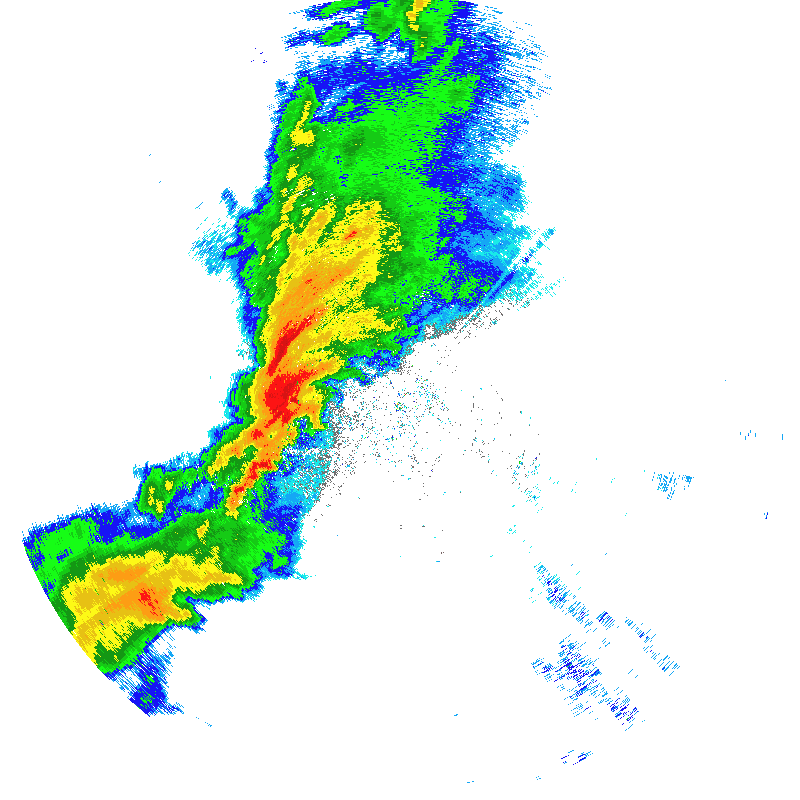
\includegraphics[width=\textwidth]{./thesis_code/plots/midlothian.tx-20180421-235141-ref.png}
		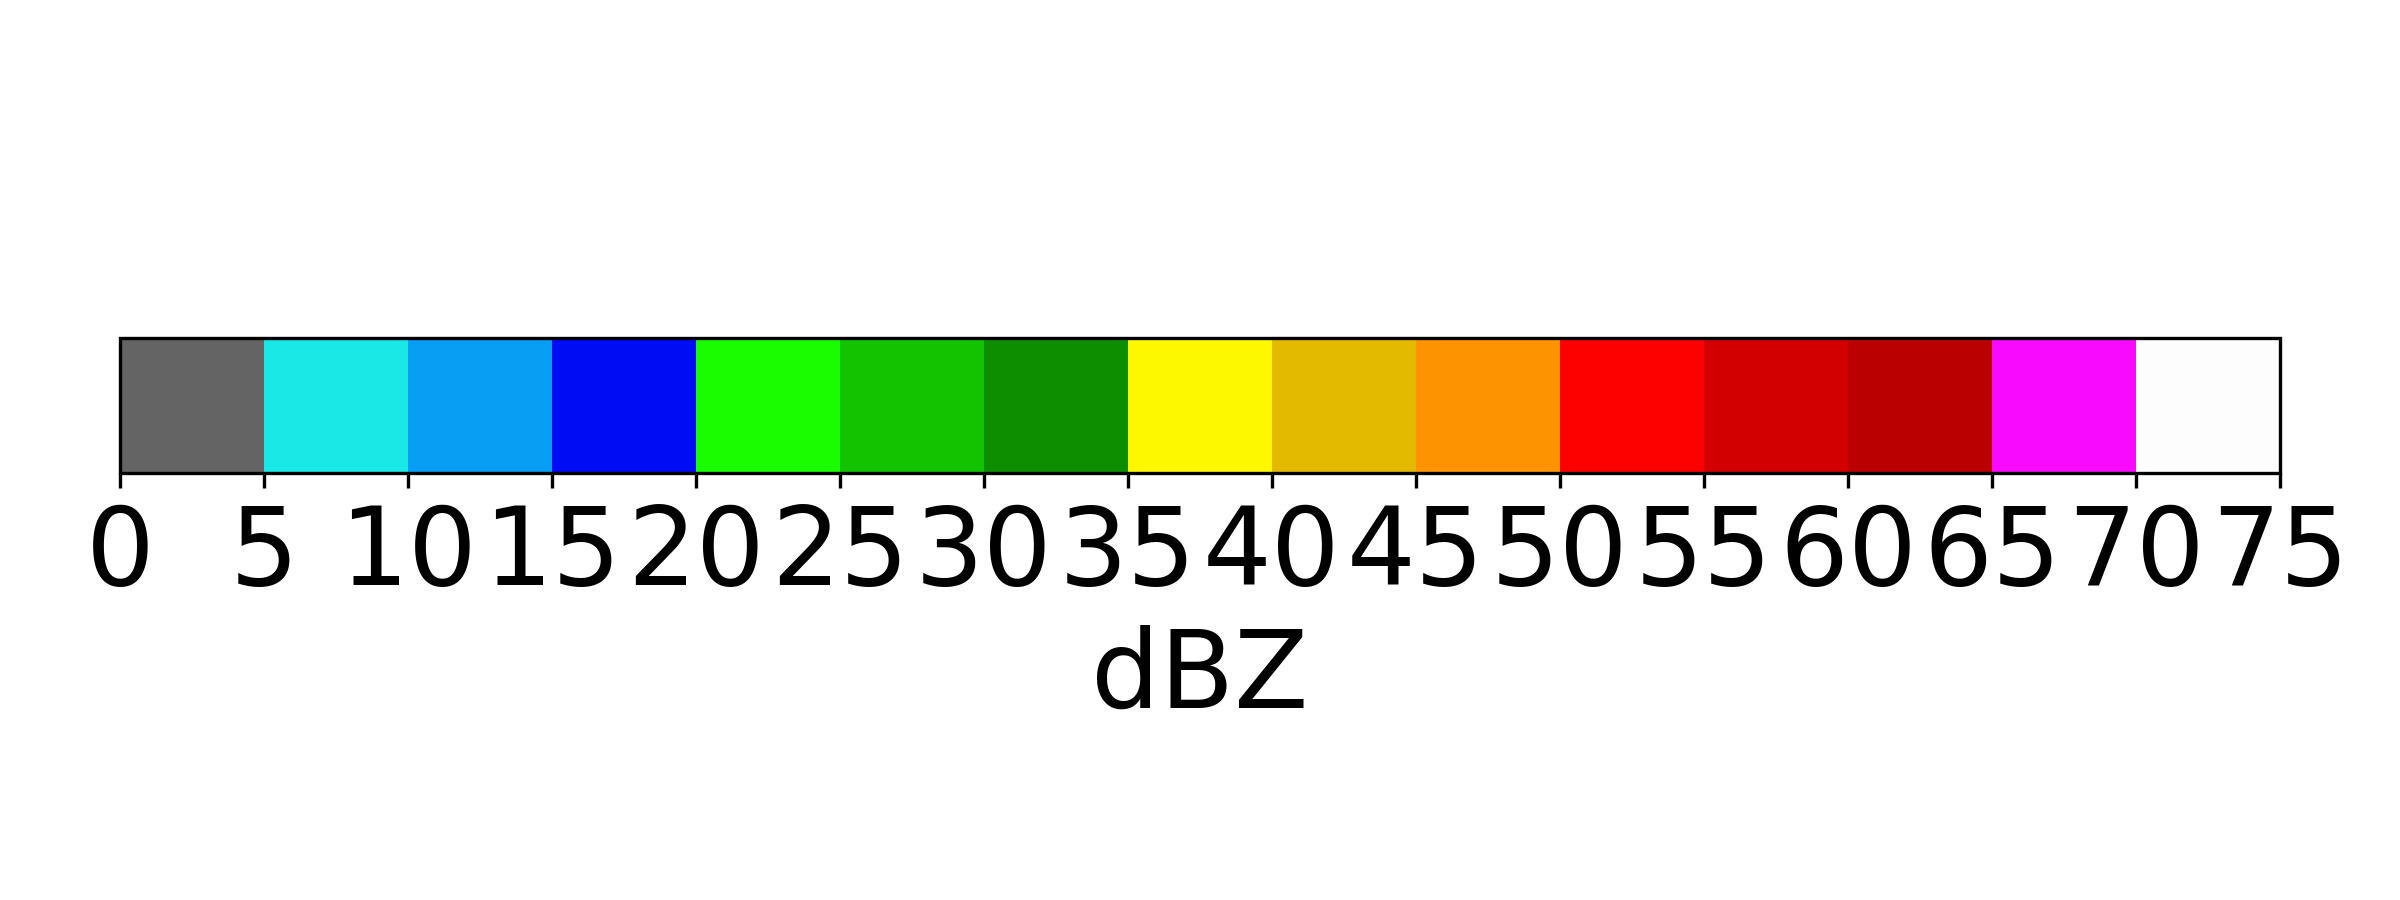
\includegraphics[width=\textwidth]{./thesis_code/plots/dfw_colormap.png}
		\caption{2018-04-21 23:51:41 UTC}
		\label{fig:bestmodel_translation2}
	\end{subfigure}
	\begin{subfigure}[b]{0.3\textwidth}
		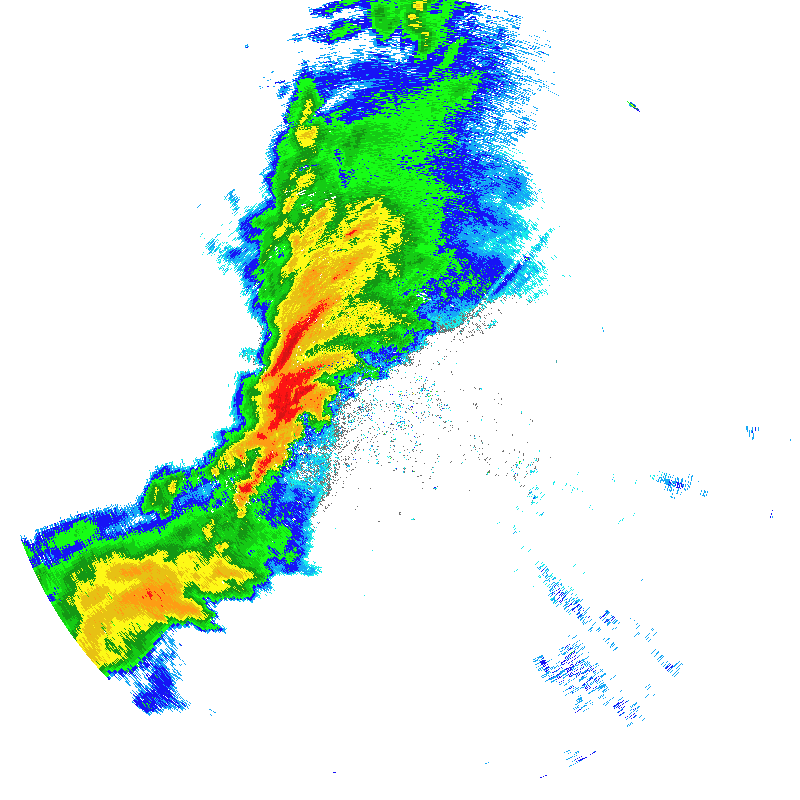
\includegraphics[width=\textwidth]{./thesis_code/plots/midlothian.tx-20180421-235238-ref.png}
		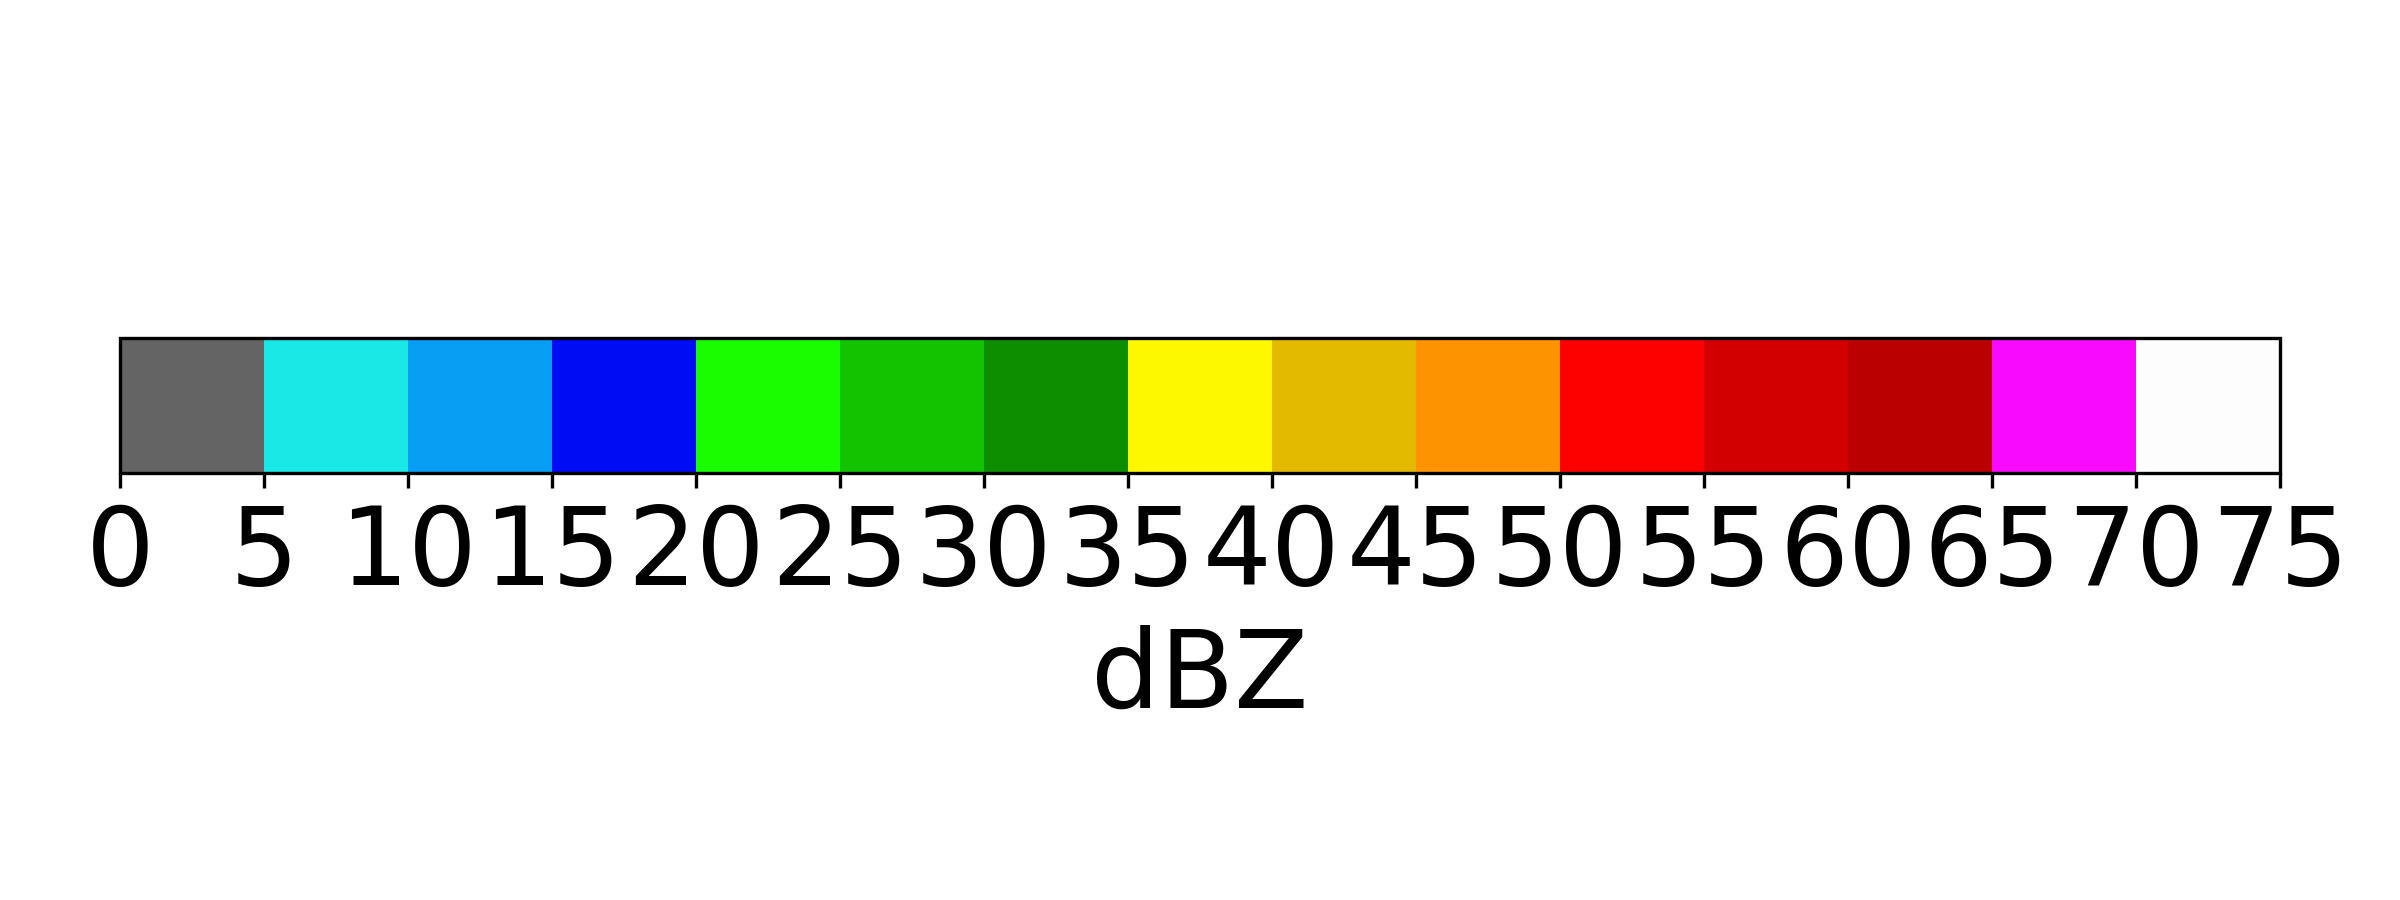
\includegraphics[width=\textwidth]{./thesis_code/plots/dfw_colormap.png}
		\caption{2018-04-21 23:52:38 UTC}
		\label{fig:bestmodel_translation3}
	\end{subfigure}
	\\
	\begin{subfigure}[b]{0.3\textwidth}
		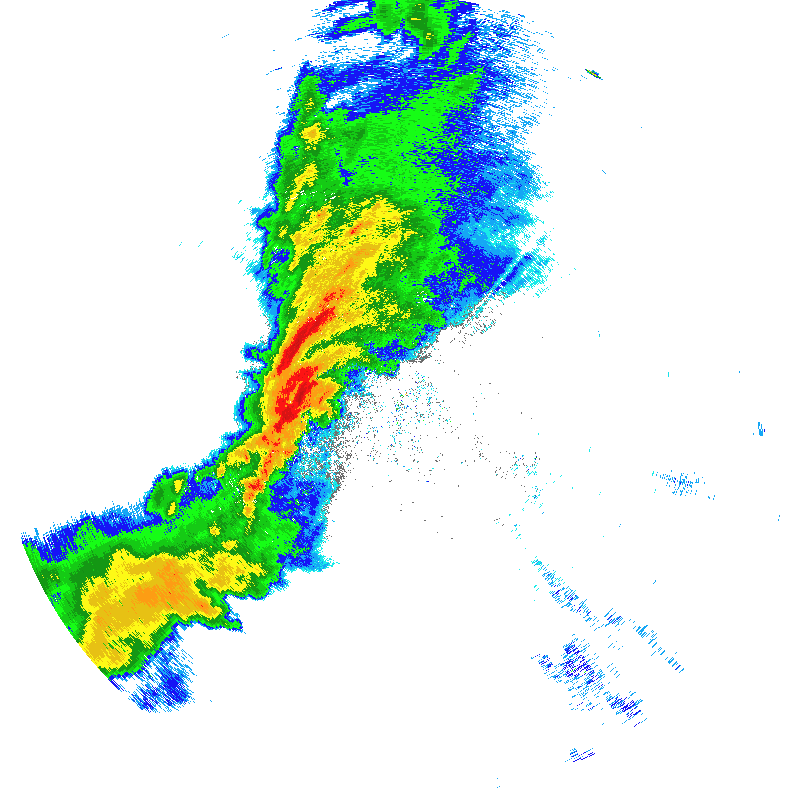
\includegraphics[width=\textwidth]{./thesis_code/plots/midlothian.tx-20180421-235338-ref.png}
		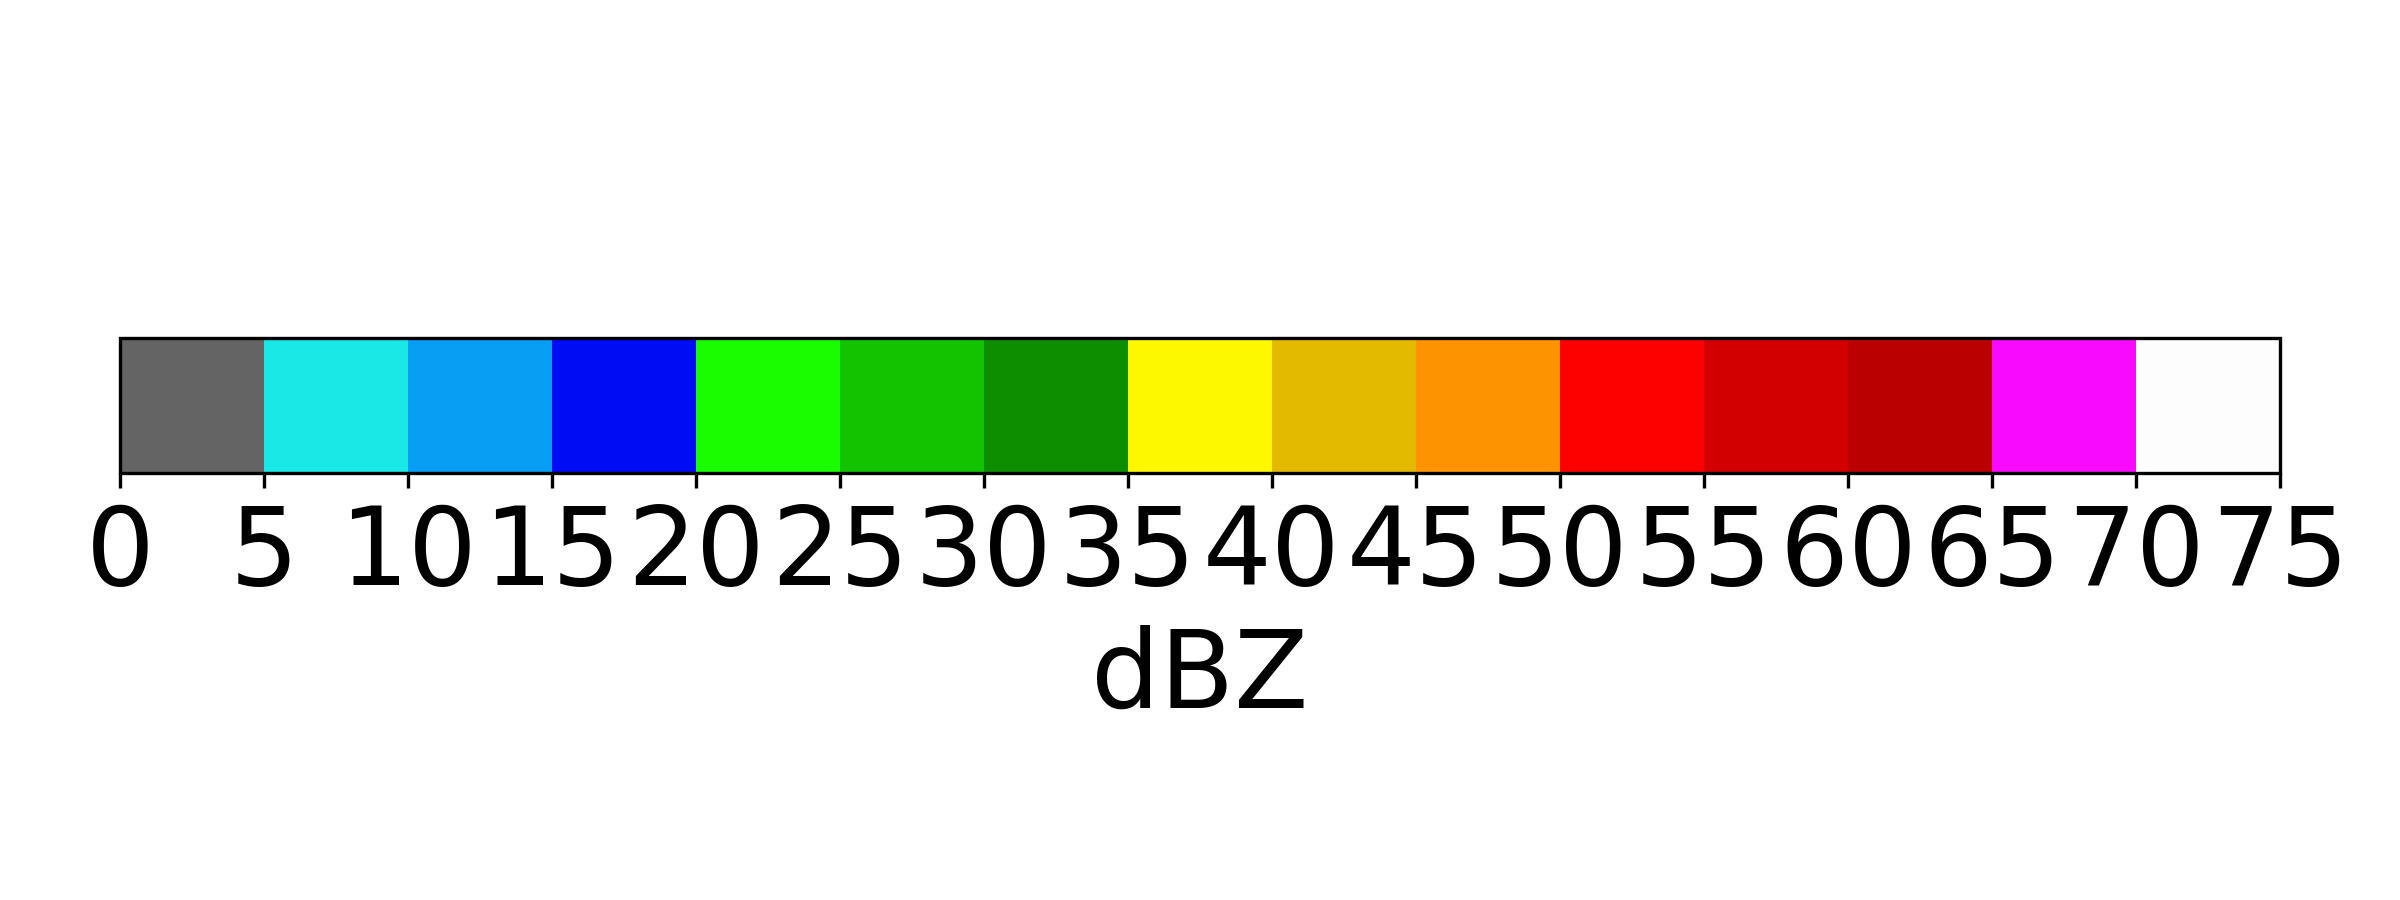
\includegraphics[width=\textwidth]{./thesis_code/plots/dfw_colormap.png}
		\caption{2018-04-21 23:53:38 UTC}
		\label{fig:bestmodel_translation4}
	\end{subfigure}
	\begin{subfigure}[b]{0.3\textwidth}
		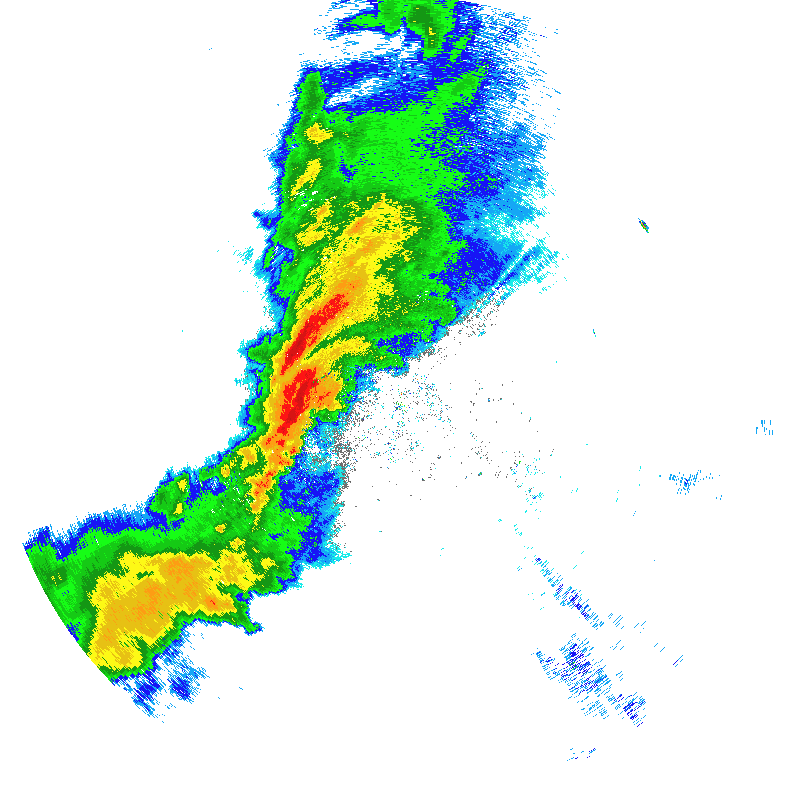
\includegraphics[width=\textwidth]{./thesis_code/plots/midlothian.tx-20180421-235438-ref.png}
		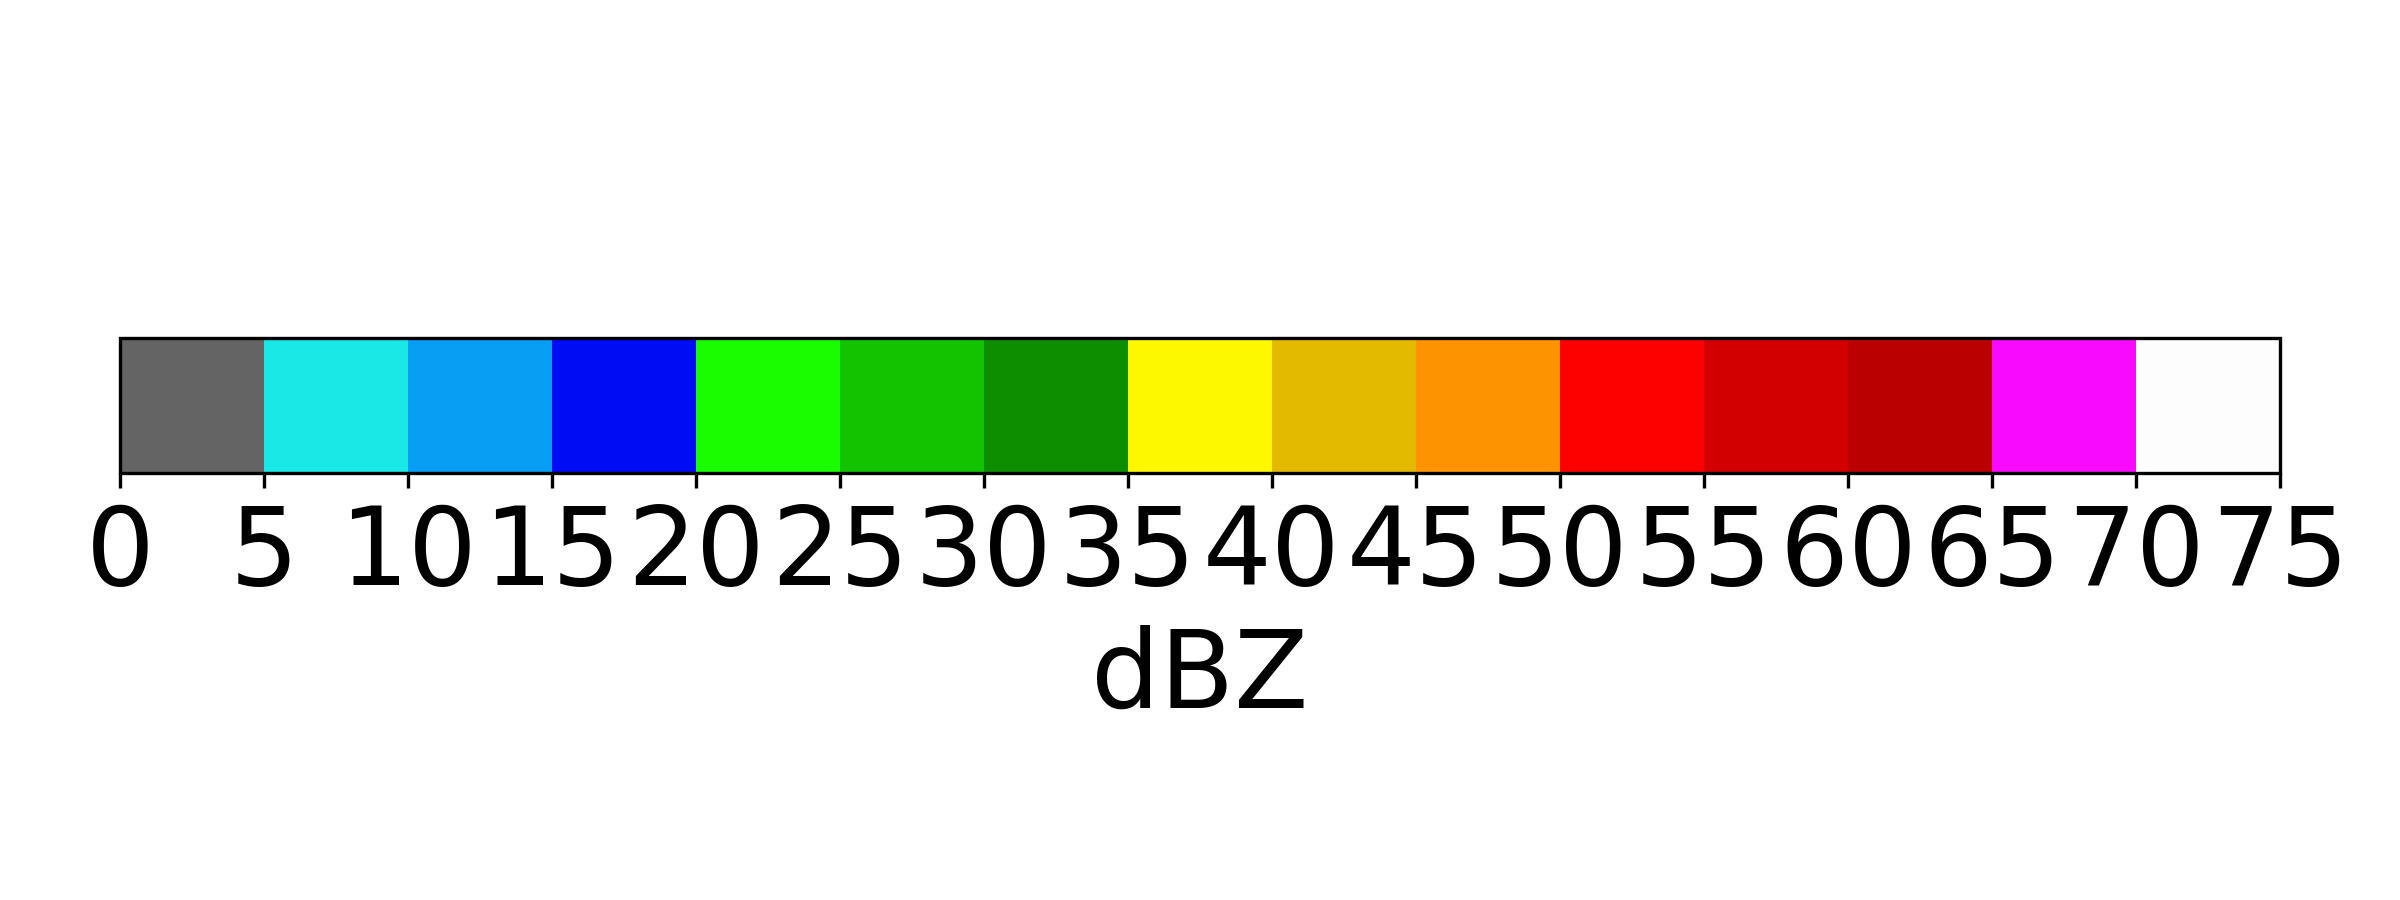
\includegraphics[width=\textwidth]{./thesis_code/plots/dfw_colormap.png}
		\caption{2018-04-21 23:54:38 UTC}
		\label{fig:bestmodel_translation5}
	\end{subfigure}
	\begin{subfigure}[b]{0.3\textwidth}
		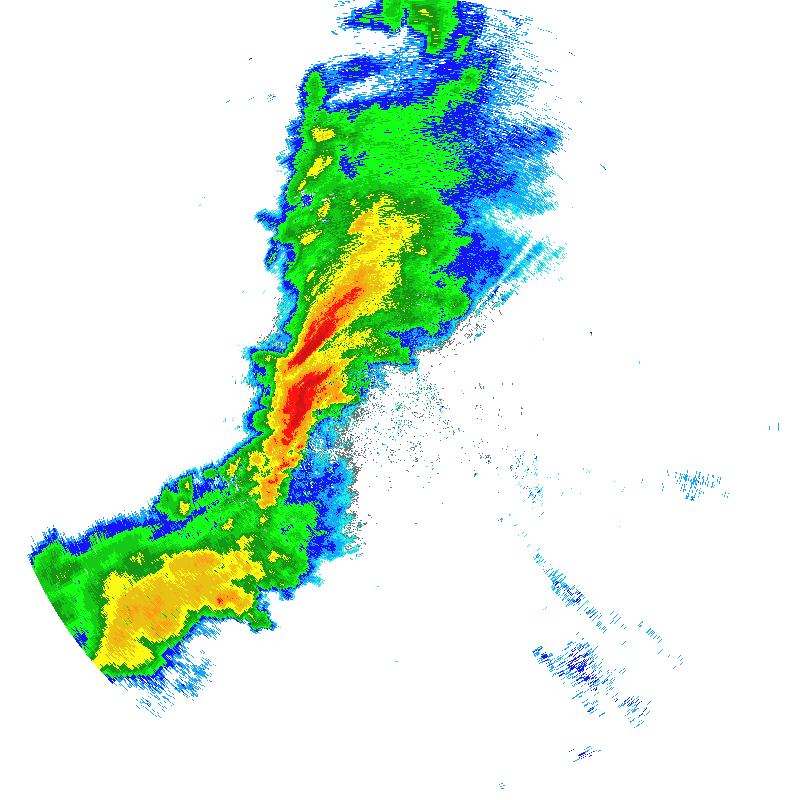
\includegraphics[width=\textwidth]{./thesis_code/plots/midlothian.tx-20180421-235538-ref.png}
		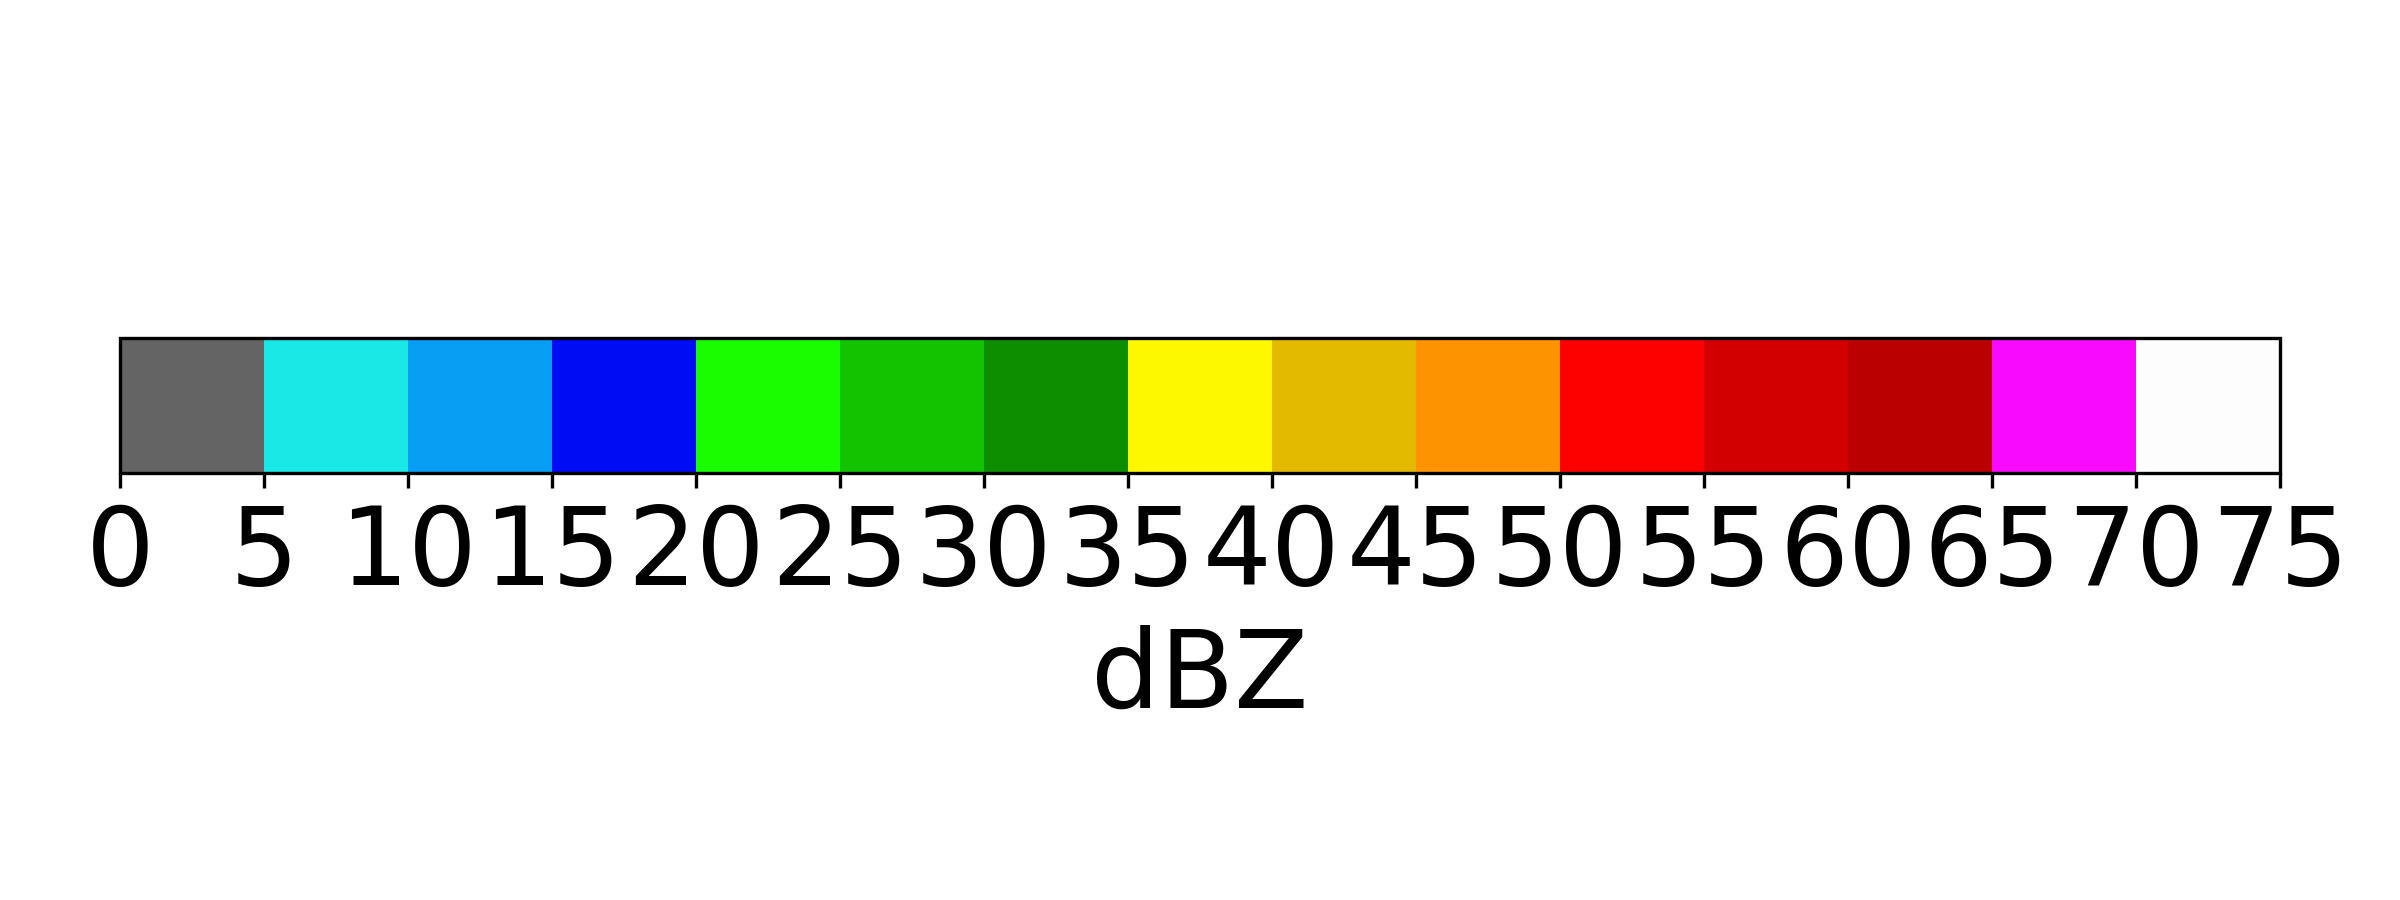
\includegraphics[width=\textwidth]{./thesis_code/plots/dfw_colormap.png}
		\caption{2018-04-21 23:55:38 UTC}
		\label{fig:bestmodel_translation6}
	\end{subfigure}
	\caption{A particular precipitation event as observed in successive scans. Note the similarity between successive scans. In an ideal classifier, all would be classified as "Convective."}
	\label{fig:bestmodel_translation}
\end{figure}

Convolutional neural networks like VGG16 are designed to be resilient to this type of translation, but a recent paper \cite{zhang2019making} illustrated that by replacing the downsampling layer which follows a convolution block, we can gain both accuracy and consistency of prediction.
This layer is called BlurPool, as it is a pooling layer that utilizes a Gaussian blur filter kernel to first low-pass filter the image feature representations following a particular convolution block, before applying the downsampling mechanism.

An important step in any deep learning classifier is the downsampling layer, which takes as input a wider, shallower set of image representations, and reduces the width while increasing the depth.
Width in this context refers to what can be thought of as the number of pixels in the image or image representation, and depth, the number of channels or activations.
We wish to take a high-dimensional input (image), and produce a low dimensional set of predictions (classes).
Thus, these downsampling layers are of critical importance to the deep learning process.

The authors of this paper argue that the current set of most commonly used downsampling layers, however, is not as resilient to translation in input image objects as would be desirable.
They draw inspiration from signal processing, whereby a signal must be low-pass filtered prior to down-sampling, to mitigate issues arising from potential high frequency energy aliasing into lower frequencies.
The current most often used downsampling layers in deep learning models, like max pooling or average pooling, essentially allow this sort of aliasing.
With a Gaussian filter kernel applied to activation layers prior to  downsampling, we can mitigate or eliminate this type of contamination, effectively anti-aliasing the deep learning operations and promoting shift-invariance in the model.

\section{BatchNormalization}
\label{sec:bestmodel_batchnorm}

We have presented some treatment of the Batch Normalization process elsewhere, though this section aims to more deeply describe its place in deep learning model research, its added value for this effort, and some implementation strategies used to adapt the off-the-shelf VGG16 architecture to include Batch Normalization in its convolution blocks.

As described above, the batch normalization, or BatchNorm or BN, layer seeks to normalize and standardize the activations in deep neural networks in order to minimize the effects of covariance shift and reduce issues arising from vanishing and exploding gradients.
This effect is confirmed in \cite{bjorck2018understanding}, who illustrates several interesting features of BN in deep neural networks. 
One insight gained was in examining activation weight ratios in intermediate layers in DNNs trained both with and without BN. 
Those trained with BN had much larger ratios and more variable values in gradients than did the DNN trained without BN.
This indicates that without BN, activations tend to converge to the same values regardless of the input data, indicating a covariate shift.
With BN, however, the data more deeply influences intermediate layers.
Additionally, it was shown that empirical distributions of gradient values with BN exhibited a distribution more reminiscent of a Gaussian curve, lower kurtosis, and slimmer tails, which shows that the gradient values were more clustered around the mean value of zero.
Furthermore, it was demonstrated that gradient update step size created less divergence in the relative loss functions across many mini-batch sizes.
This result validates our usage of a variable learning parameter mechanism in part, since the loss is not adversely affected for decreasing step size.
Finally, it was shown that weights in intermediate layers tended to converge to low-rank, more variable values in the DNN without BN, whereas the DNN trained with BN had a less marked effect in these terms.

Theoretically, it seems clear that batch normalization layers can and will help in our experiment as well, but there is also a large corpus of practical evidence to support this hypothesis as well.
The fundamental VGG16 architecture \cite{simonyan2014very} that we have built our base architecture upon was chosen for its demonstrated success in transferring learning effectively to target tasks that were much different than source tasks, but as it was introduced in 2014, the model does not include any BN layers, since they had not yet been discovered.
The paper also introduced a variation called VGG19, which included more layers and represented a larger network, but again, it did not include BN.

The Extreme Inception, or Xception, DNN includes batch normalization in all convolution and separable convlution layers \cite{chollet2017xception}.
It was based in part on a style of network called \textit{Inception}, of which there exist multiple versions.
The third major version of this network, InceptionV3, batch normalizes all output activations \cite{szegedy2016rethinking}.
Another iteration of this style of network involves its combination with the ResNet style of architecture, and the combination, referred to as Inception-ResNet, includes some BN layers \cite{szegedy2017inception}.
This is of particular interest, since the authors implemented their network using Tensorflow \cite{tensorflow2015-whitepaper}, and discovered that implementing BN for every activation layer led to greatly increased memory usage and slower speed.
Our networks also use Tensorflow, and our results indicate a similar effect, where networks with BN spent more time in training and necessitated a smaller mini-batch size.
However, BN was still utilized where it was deemed reasonable and necessary to do so.

One final class of deep neural network that is worth mentioning is the MobileNet \cite{howard2017mobilenets}.
These networks take their name from their intended use space; mobile devices.
On such devices, trained networks must have a lower data footprint.
This makes these networks applicable to situations and modalities where compute-limited or otherwise costrained compute systems must be used, as in Internet of Things sensor setups.
This comes at a cost of accuracy and precision in learning classifiable deep feature representations, and in preliminary testing, our VGG16 convolutional base outperformed MobileNet feature extractors.
Still, it is important to note that in MobileNets, BN is present.

We thus consider batch normalization to be a necessary layer to add to our architecture, and we will illustrate an experiment below that compares networks with and without BN and demonstrates the layer's efficacy in improving classifications.

\section{Experiment Setup}
\label{sec:bestmodel_experiment}

The diagram in Figure \ref{fig:end-to-end} demonstrates the architecture configuration we use in this set of experiments.
We included both BlurPool and batch normalization layers in the diagram to illustrate where these layers would exist in certain configurations.

The goal of this experiment is to test the end-to-end deep learning model to discover the optimal set of parameters and hyperparameters for the expanded weather radar image dataset.
There are a few differences from the earlier experiments presented in this work:

\begin{itemize}
	\item Increased dataset;
	\item Usage of batch normalization layers;
	\item Downsampling via BlurPool layers, and;
	\item Implementation strategy.
\end{itemize}

We have detailed above the efforts to increase the dataset using data from 2018 and performing first stage classifications with the deep neural network presented in Chapter \ref{sec:classifying}.
This experiment will seek to test the effectiveness of using BN layers after each activation to manage gradients and reduce covariate shift, while also comparing the performance of low-pass filtered, shift-invariant downsampling operations of BlurPool with the default average or max pooling operations predominant in most off-the-shelf deep neural networks.
Finally, this approach involves a deeper implementation strategy in Tensorflow, whereby the BlurPool activation was developed from scratch, and the BN layers were added via custom inclusion to all convolutional layers in the feature extractor portion of the end-to-end model architecture.

Specifically, we tested nine configurations, as shown in Table \ref{table:bestmodel_experiment_results}.
As can be seen, the BlurPool parameter of \textit{kernel size} governs the filter kernel that is used to perform the downsampling operation.
A kernel size of 1 produces a 1x1 convolution and thus, offers no desirable filtering characteristics.
The kernel size of 2 yields a 2x2 filter kernel that is essentially an average pooling operation, which gives a useful comparison to an industry-standard downsampling mechanism.
The kernel BlurPool (k=2) is given by:

\[
k=\frac{1}{N}
	\begin{bmatrix}
	1 & 1 \\
	1 & 1
	\end{bmatrix}
\]

where $N$ is given by the sum of all elements in the matrix. Here, $N=4$.

The kernel BlurPool (k=3) is given by:

\[
k=\frac{1}{N}
	\begin{bmatrix}
	1 & 2 & 1 \\
	2 & 4 & 2 \\
	1 & 2 & 1	
	\end{bmatrix}
\]

The kernel BlurPool (k=5) is given by:

\[
k= \frac{1}{N}
	\begin{bmatrix}
	 1 & 4 & 6 & 4 & 1 \\
	 4 & 16 & 24 & 16 & 4 \\
	 6 & 24 & 36 & 24 & 6 \\
	 4 & 16 & 24 & 16 & 4 \\
	 1 & 4 & 6 & 4 & 1
	\end{bmatrix}
\]

The kernel BlurPool (k=7) is given by:

\[
k=\frac{1}{N}
	\begin{bmatrix}
	  1 & 6 & 15 & 20 & 15 & 6 & 1 \\
	  6 & 36 & 90 & 120 & 90 & 36 & 6 \\
	 15 & 90 & 225 & 300 & 225 & 90 & 15 \\
	 20 & 120 & 300 & 400 & 300 & 120 & 20 \\
	 15 & 90 & 225 & 300 & 225 & 90 & 15 \\ 
	  6 & 36 & 90 & 120 & 90 & 36 & 6 \\
	  1 & 6 & 15 & 20 & 15 & 6 & 1
	\end{bmatrix}
\]
% table showing results of all tests
%\begin{table*}[t]
%	\centering
%	\begin{tabular}{ccccc}
%		& & \multicolumn{3}{c}{ Three Class Averaged Classification Statistics } \\
%		Configuration Details & Name & Categorical Accuracy & Precision & Recall \\
%		\hline
%		Default VGG16 Architecture & VGG16 & 0.9208 & 0.9249 & \textbf{0.9165} \\
%		VGG16 with default convolution and BlurPool downsampling (kernel size of 2) & DC\_BP (k=2) & 0.8958 & 0.9071 & 0.8830 \\
%		VGG16 with default convolution and BlurPool downsampling (kernel size of 3) & DC\_BP (k=3) & 0.8807 & 0.8901 & 0.8720 \\
%		VGG16 with default convolution and BlurPool downsampling (kernel size of 5) & DC\_BP (k=5) & 0.9036 & 0.9143 & 0.8916 \\
%		VGG16 with default convolution and BlurPool downsampling (kernel size of 7) & DC\_BP (k=7) & 0.8946 & 0.9053 & 0.8824 \\
%		VGG16 with convolution + batch normalization and BlurPool downsampling (kernel size of 2) & BN\_BP (k=2) & 0.9160 & 0.9238 & 0.9148 \\
%		VGG16 with convolution + batch normalization and BlurPool downsampling (kernel size of 3) & BN\_BP (k=3) & 0.9160 & 0.9238 & 0.9148 \\
%		VGG16 with convolution + batch normalization and BlurPool downsampling (kernel size of 5) & BN\_BP (k=5) & \textbf{0.9220} & \textbf{0.9329} & 0.9161 \\
%		VGG16 with convolution + batch normalization and BlurPool downsampling (kernel size of 7) & BN\_BP (k=7) & 0.9198 & 0.9305 & 0.9160 \\
%		\hfill
%	\end{tabular} 
%	\caption{Comprehensive results of each deep learning configuration tested using the full dataset. The values reported reflect the class-weighted average for both Precision and Recall. The Name column matches annotations on Figure \ref{fig:precision_recall_curves}. Bolding accentuates best result in each column.}
%	\label{table:experiment_results}
%\end{table*}

\section{Results}
\label{sec:bestmodel_results}

\begin{table}[t]
	\centering
	\begin{tabular}{ccccc}
		& & \multicolumn{3}{c}{ Three Class Avg Classification Stats } \\
		Configuration Details & Name & Categorical & Precision & Recall \\
		&      & Accuracy    &           &        \\
		Default VGG16 Architecture & VGG16 & 0.9208 & 0.9249 & \textbf{0.9165} \\
		& & & & \\
		VGG16 with default convolution and & DC\_BP (k=2) & 0.8958 & 0.9071 & 0.8830 \\
		BlurPool downsampling (k=2) & & & & \\
		VGG16 with default convolution and & DC\_BP (k=3) & 0.8807 & 0.8901 & 0.8720 \\
		BlurPool downsampling (k=3) & & & & \\
		VGG16 with default convolution and & DC\_BP (k=5) & 0.9036 & 0.9143 & 0.8916 \\
		BlurPool downsampling (k=5) & & & & \\
		VGG16 with default convolution and & DC\_BP (k=7) & 0.8946 & 0.9053 & 0.8824 \\
		BlurPool downsampling (k=7) & & & & \\
		VGG16 with convolution + BatchNorm & BN\_BP (k=2) & 0.9160 & 0.9238 & 0.9148 \\
		and BlurPool downsampling (k=2) & & & & \\
		VGG16 with convolution + BatchNorm & BN\_BP (k=3) & 0.9160 & 0.9238 & 0.9148 \\
		and BlurPool downsampling (k=3) & & & & \\
		VGG16 with convolution + BatchNorm & BN\_BP (k=5) & \textbf{0.9220} & \textbf{0.9329} & 0.9161 \\
		and BlurPool downsampling (k=5) & & & & \\
		VGG16 with convolution + Batch Norm & BN\_BP (k=7) & 0.9198 & 0.9305 & 0.9160 \\
		and BlurPool downsampling (k=7) & & & & \\
	\end{tabular}
	\caption{Comprehensive results of each deep learning configuration tested using the full dataset. The values reported reflect the class-weighted average for both Precision and Recall. The Name column matches annotations on Figure \ref{fig:bestmodel_precision_recall_curves}. Bolding accentuates best result in each column.}
	\label{table:experiment_results}
\end{table}

\begin{figure}[!t]
	\centering
	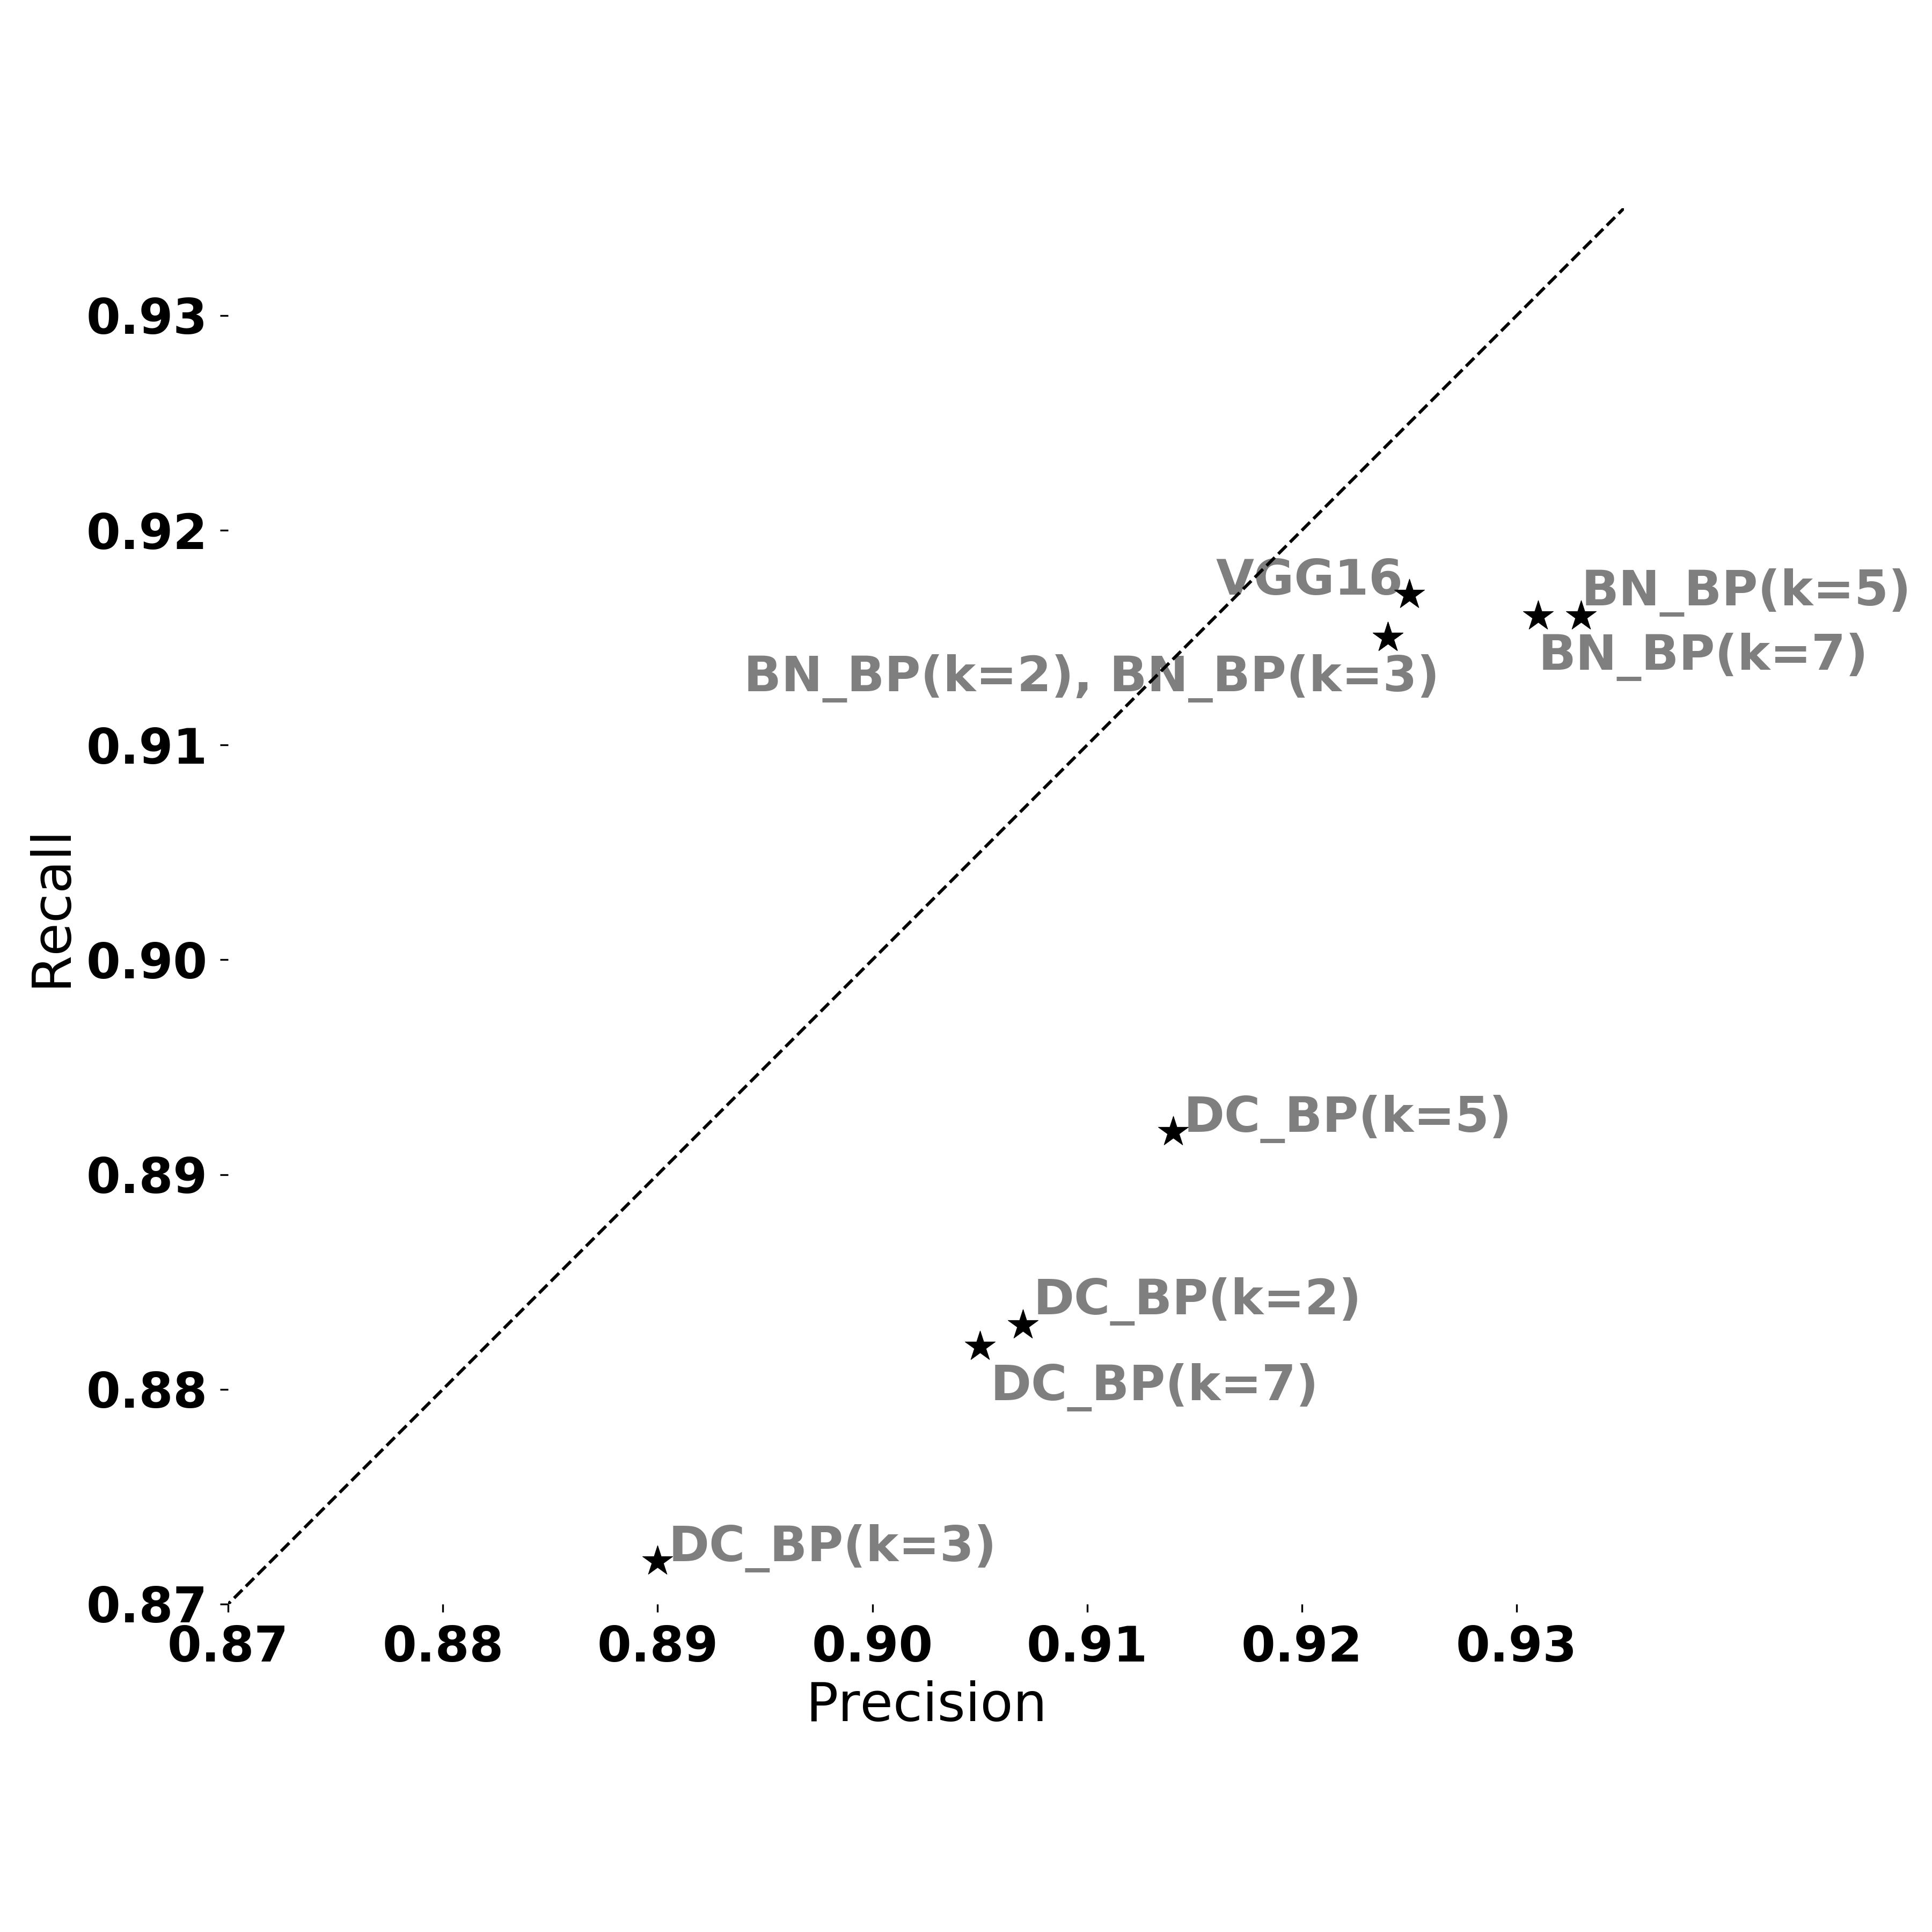
\includegraphics[width=0.85\textwidth]{./thesis_code/plots/precision_recall_curve_all_configs_bw.png}
	\caption{Precision and Recall statistics for each configuration tested. See Table \ref{table:experiment_results} for configurations corresponding to the names in this figure.}
	\label{fig:bestmodel_precision_recall_curves}
\end{figure}

\begin{figure}[h]
	\centering
	\begin{subfigure}[b]{0.45\textwidth}
		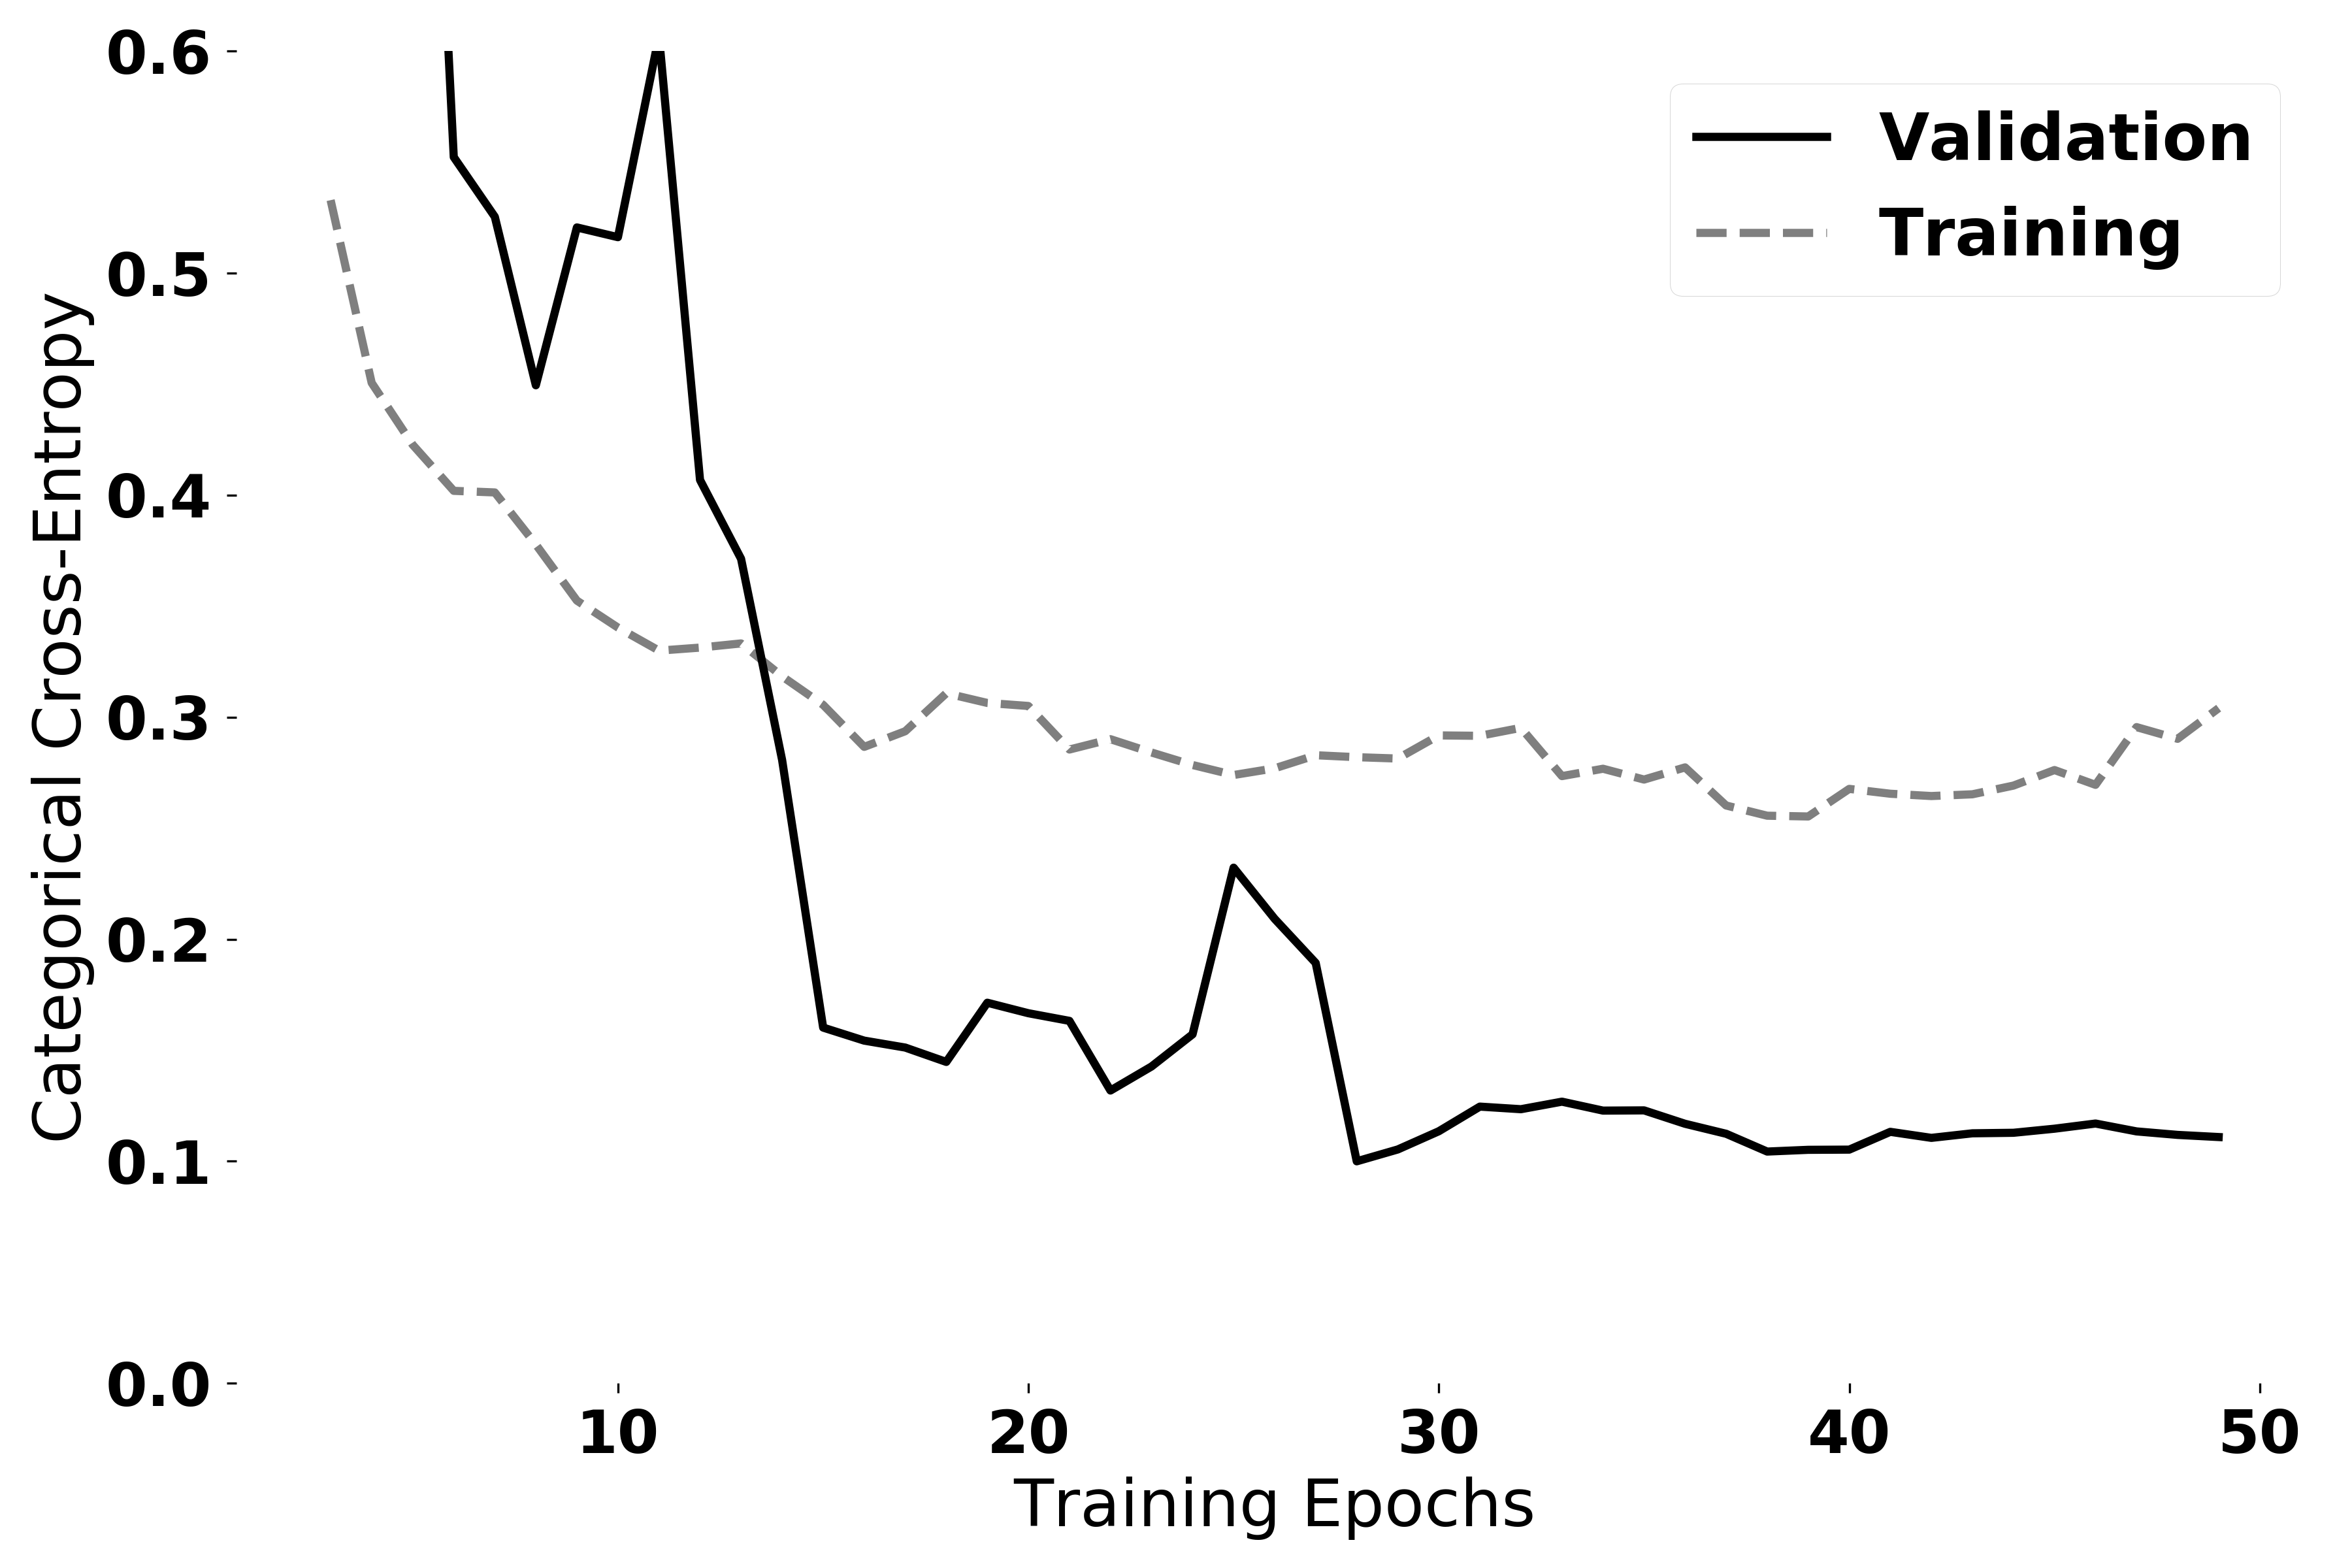
\includegraphics[width=\textwidth]{./thesis_code/plots/20191011_BP_k5_BN_loss_bw.png}
		\caption{Loss}
		\label{fig:bestmodel_first_case}
	\end{subfigure}
	\begin{subfigure}[b]{0.45\textwidth}
		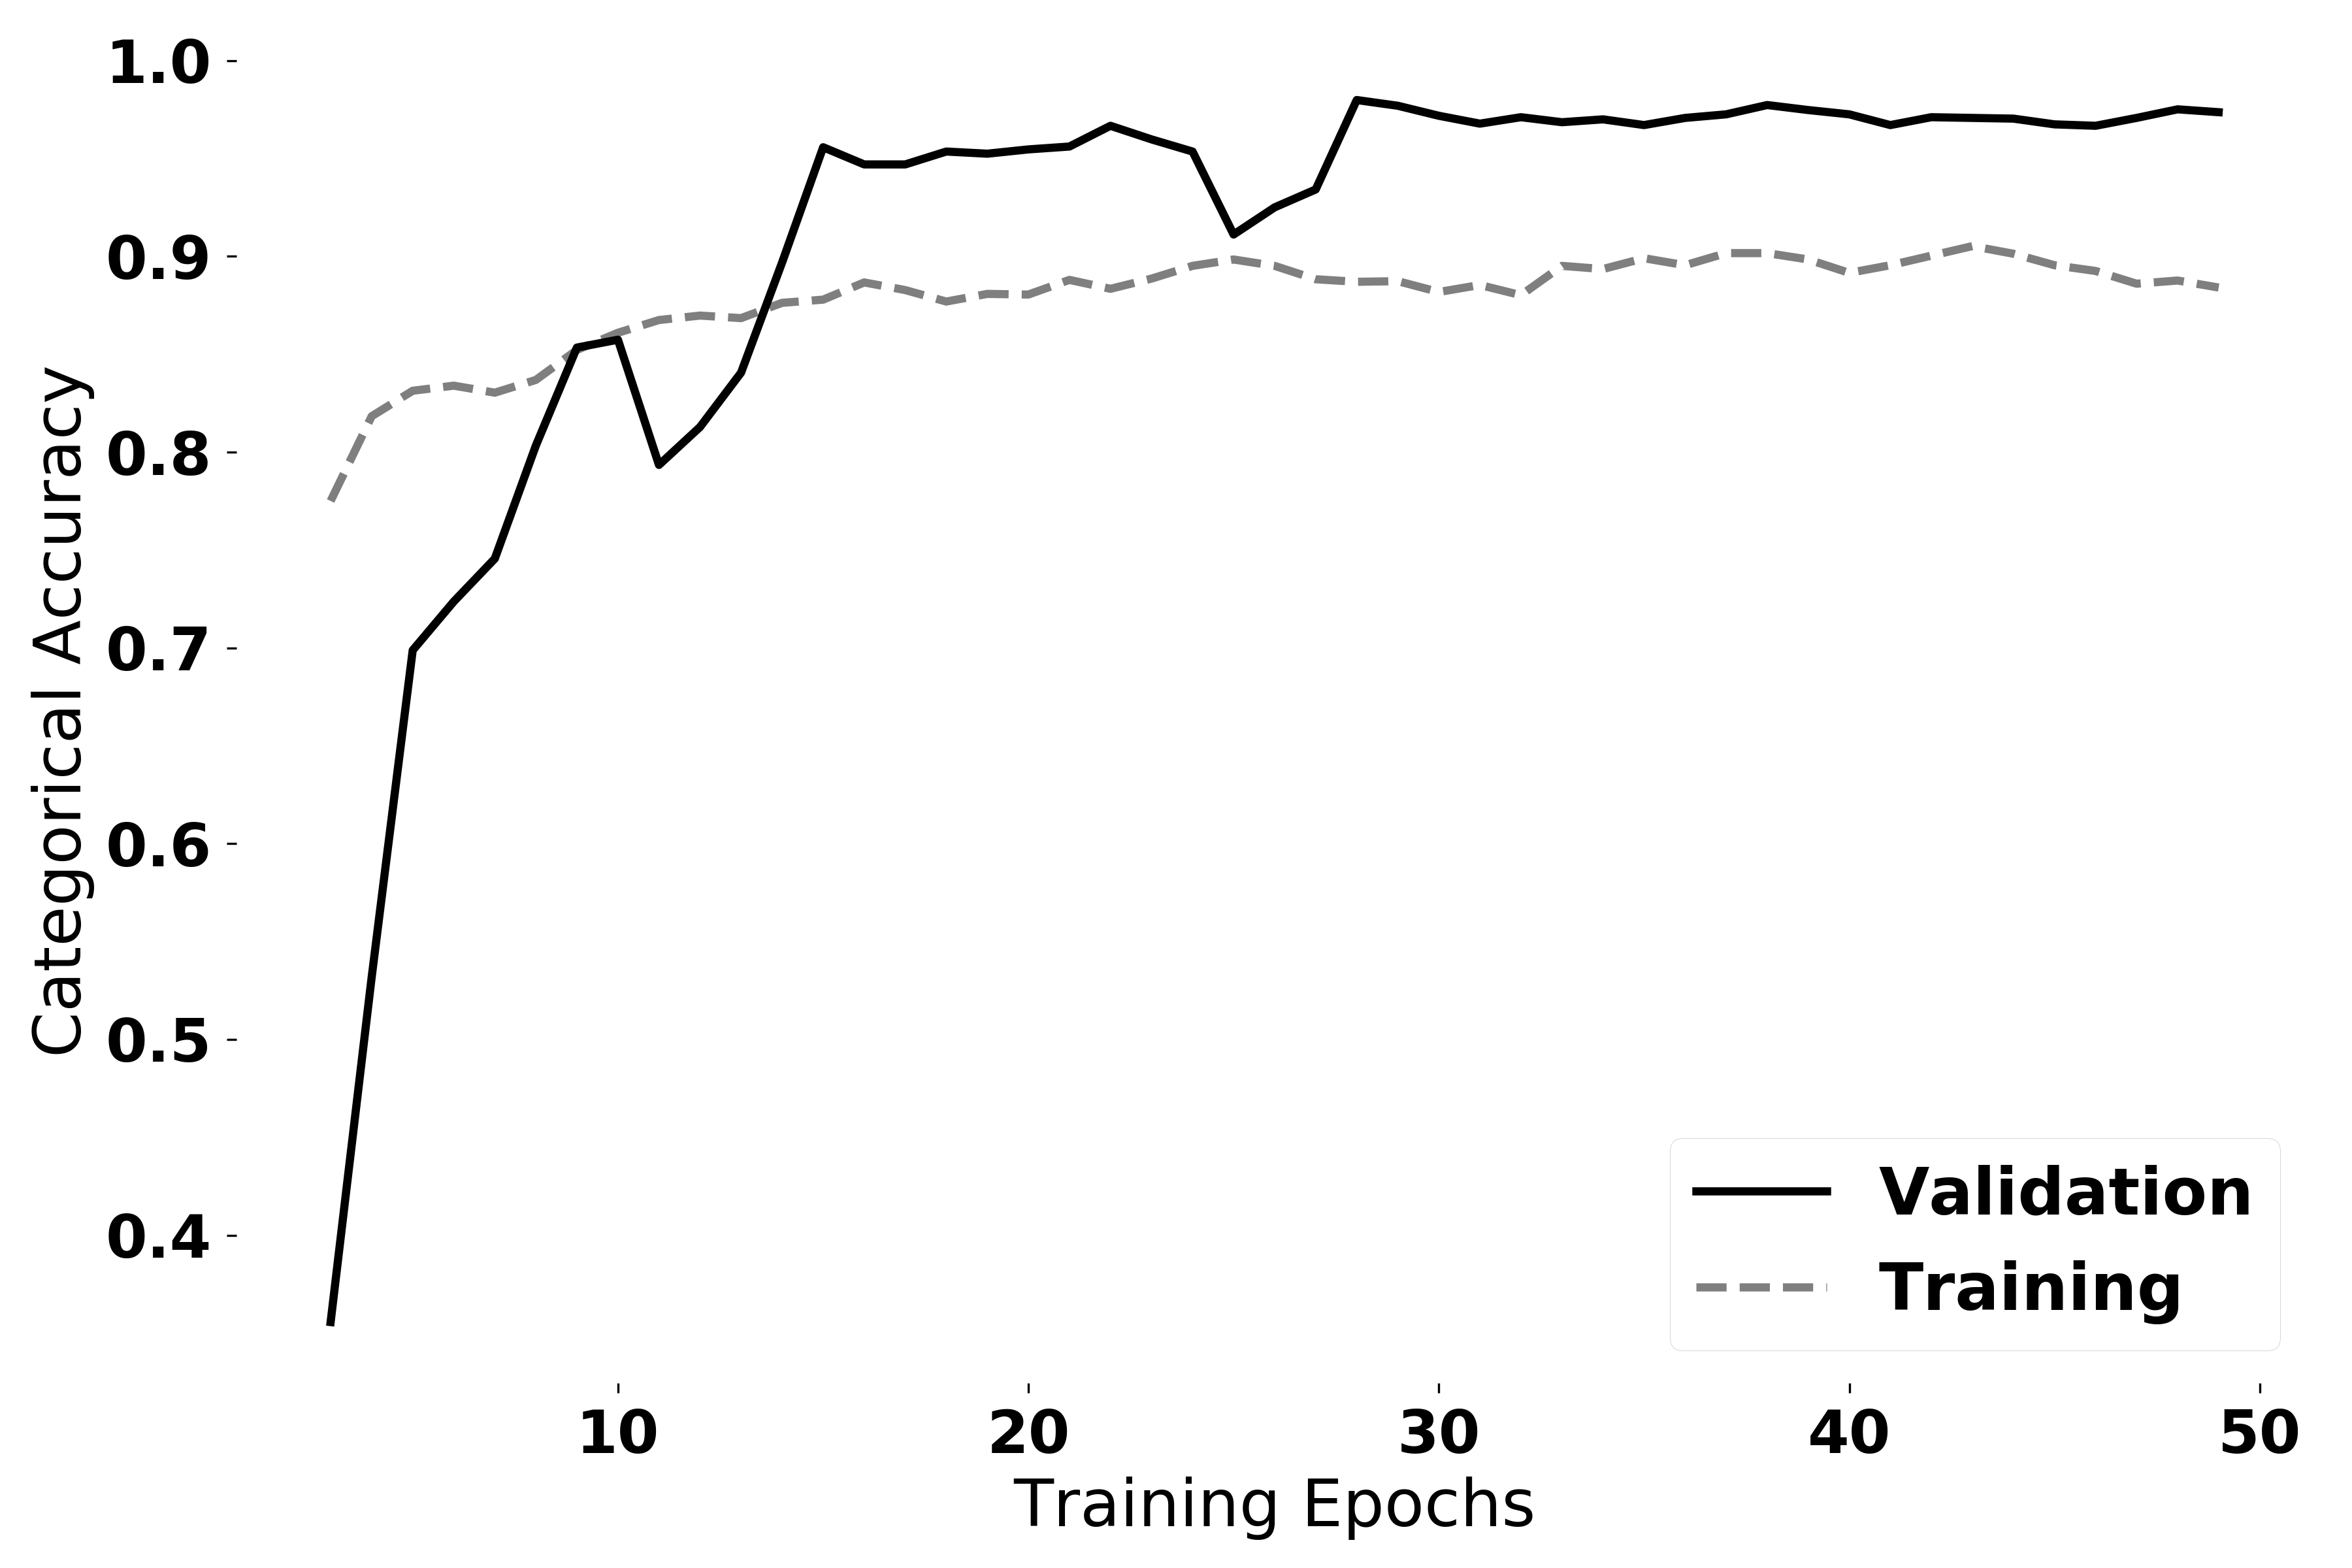
\includegraphics[width=\textwidth]{./thesis_code/plots/20191011_BP_k5_BN_acc_bw.png}
		\caption{Accuracy}
		\label{fig:bestmodel_second_case}
	\end{subfigure}
	\caption{Loss and accuracy curves for our best-case network, which utilized the VGG16 base model feature extractor, with batch normalization layers following each convolutional layer, and BlurPool layers with a kernel size of 5. Training was allowed to progress with base model weights frozen until a loss plateau was reached, before fine-tuning by allowing all parameters to update during training. Fine Tuning began at Epoch 36.}
	\label{fig:bestmodel_fig_sim}
\end{figure}

The results of the described experiments can be seen in Table \ref{table:experiment_results}.
Interestingly, the default configuration given by VGG16 yields very good results, and indeed, has the highest Recall value of any configuration tested.
However, the best overall architecture was that which utilized both batch normalization and BlurPool (k=5).
It registered the highest categorical accuracy as well as the highest precision, and its recall was nearly equivalent to the best-in-class default VGG16.

\section{Classifications on Unseen Data}
\label{sec:bestmodel_newdata}

\begin{figure}[!t]
	\centering
	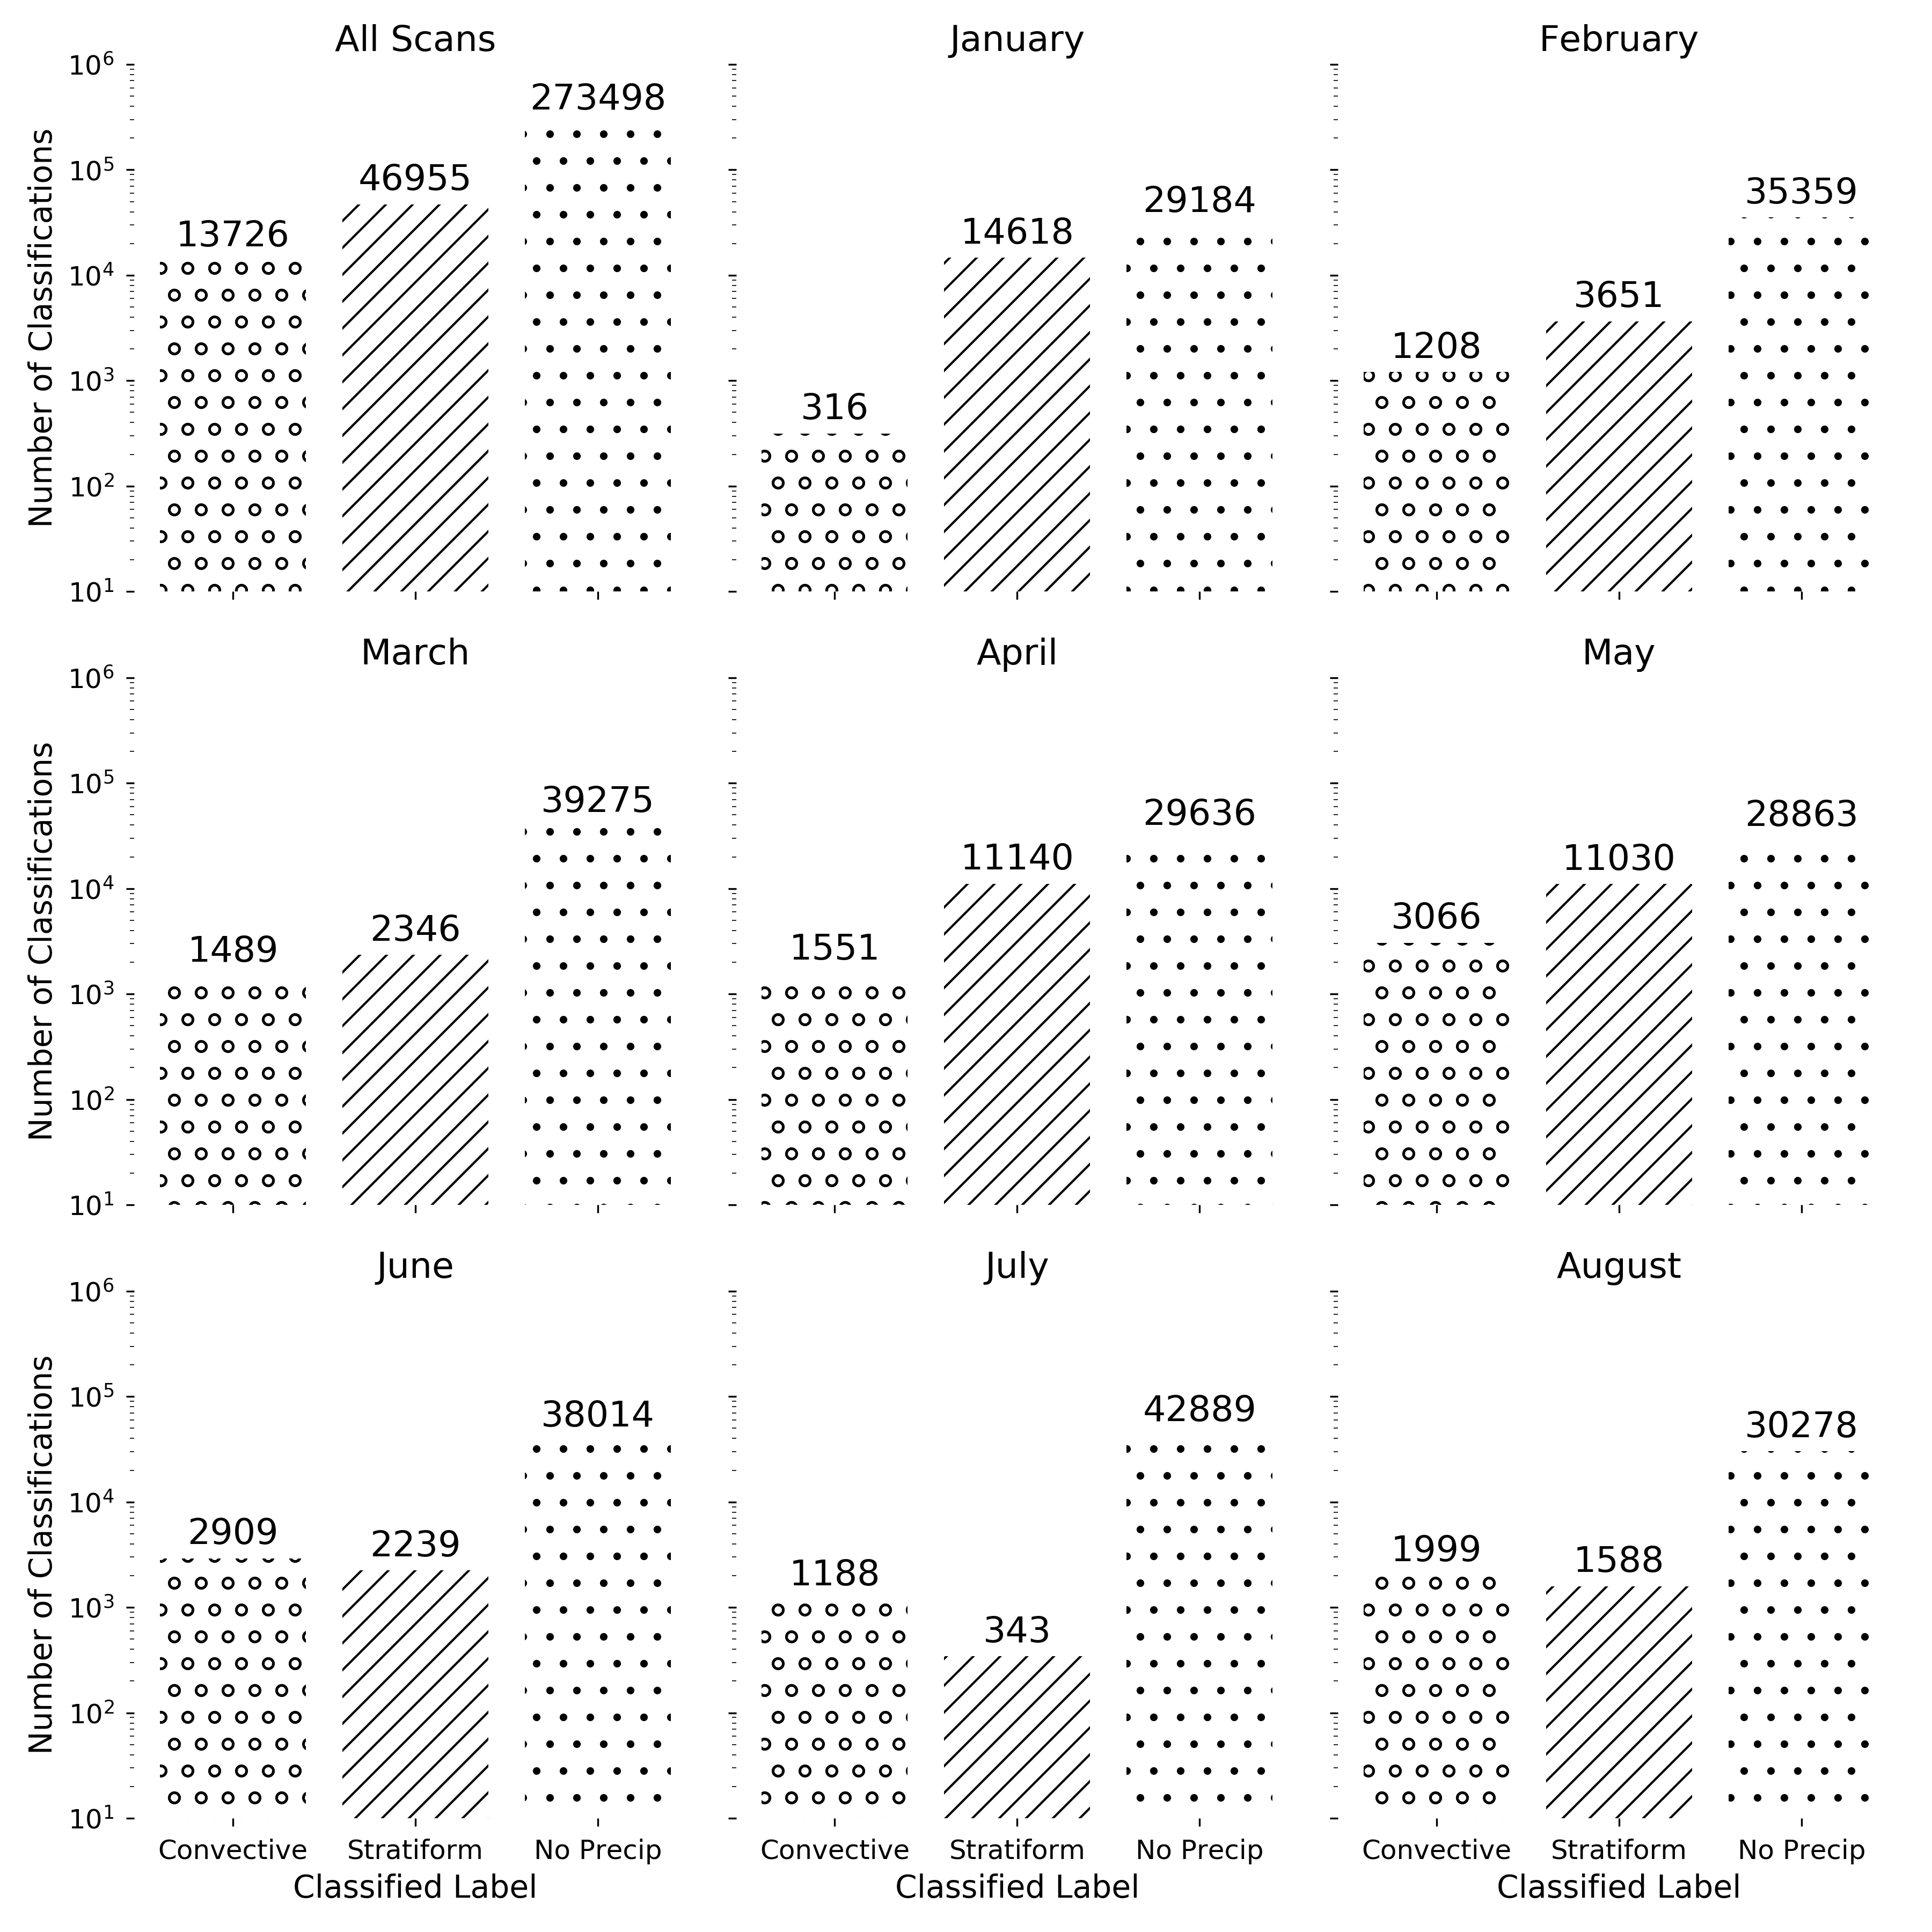
\includegraphics[width=\textwidth]{./thesis_code/plots/2019_predictions_hist_bw.png}
	\caption{The fully trained model was deployed on all scans available from 2019 observed and recorded by the CASA XMDL radar. This set of plots shows the statistics on how images were classified for all months together (top left), and each month individually.}
	\label{fig:bestmodel_all_hists}
\end{figure}

\section{Summary}
\label{sec:bestmodel_summary}

As seen above, the added data has led to a greater level of generalization ability for the deep neural network architecture.
The addition of BlurPool appears to help not only the consistency and generalizability of the model, but also the classification accuracy.
Batch Normalization ensures the training parameters are well-behaved and thus converge to a better minimum in the loss function.
And the newly trained model quickly and efficiently produces believable classifications on large amounts of data in a short period of time.


